\documentclass[12pt, a4paper, bibliography=notnumbered]{scrreprt}
\usepackage[utf8]{inputenc}
\usepackage[hidelinks]{hyperref}
\usepackage{xurl}
\usepackage{listings}
\usepackage{FiraSans}
\usepackage{palatino}
\usepackage[T1]{fontenc}  % Correct formatting for >, <, |, etc.
\usepackage{FiraMono}  % Keep last to maintain monospace font
\usepackage{xcolor}
\usepackage{parskip}
\usepackage[multiple]{footmisc}
\usepackage{skak}
\usepackage[noabbrev,capitalise,nameinlink]{cleveref}
\usepackage[font=itshape]{quoting}

\definecolor{background}{rgb}{0.97, 0.97, 0.97}
\definecolor{comments}{rgb}{0.0, 0.64, 0.0}
\definecolor{keywords}{rgb}{0.0, 0.0, 0.64}
\definecolor{identifiers}{rgb}{0.63, 0.81, 0.94}
\definecolor{strings}{rgb}{1.0, 0.3, 0.0}

\lstset{
    language=haskell,
    basicstyle=\footnotesize\ttfamily,
    backgroundcolor=\color{background},
    keywordstyle=\color{keywords}\bfseries,
    commentstyle=\color{comments}\textit,
    stringstyle=\color{strings},
    % identifierstyle=\color{identifiers},
    breakatwhitespace=true,
    breaklines=true,
    keepspaces=true,
    captionpos=b,
    frame=tlbr,    % Margin at all 4 sides
    framesep=4pt,  % Margin size
    framerule=0pt,
    morekeywords={Eval, Exp, family, instance},
    deletekeywords={map, and, error, take}
}

\RedeclareSectionCommands[
  afterskip=1sp
]{paragraph,subparagraph}

\setkomafont{sectioning}{\firamedium}

% Line spacing
\renewcommand{\baselinestretch}{1.2}

% Change abstract appearance
\renewenvironment{abstract}
 {\small
  \begin{center}
  \bfseries \textit{\abstractname}\vspace{-.5em}\vspace{0pt}
  \end{center}
  \quotation}
 {\endquotation}

% Custom command for all inline code styling
\newcommand{\inline}[1]{\lstinline[basicstyle=\ttfamily\footnotesize]{#1}}

\title{Chesskell: Embedding a Two-Player Game in Haskell's type system}
\author{Toby Bailey}
\date{\today}

\begin{document}

\begin{titlepage}
    \maketitle
\end{titlepage}

\phantomsection
\addcontentsline{toc}{chapter}{Abstract}
\begin{abstract}
    Type-level programming allows programmers to express computation within the types of their programs. Through the use of extensions to Haskell's type system as implemented in the Glasgow Haskell Compiler (GHC), rules can be statically imposed on code to ensure that if it compiles, then it exhibits (or conversely, will not exhibit) specific behaviour. However, for these extensions to see mainstream adoption, their use in complex applications has to be practical.

    We present Chesskell, an EDSL for describing Chess games where a type-level model of the full FIDE ruleset prevents us from expressing games with invalid moves. Our work highlights current limitations when using GHC to express such complex rules due to the resulting memory usage and compile times, which we report on. We further present some approaches for working around those limitations, where possible.

    \textbf{\textit{Keywords:}} Type-level Programming, Haskell, Chess, EDSL.
\end{abstract}

{
    \newpage  % So that \phantomsection lines up nicely
    \phantomsection
    \addcontentsline{toc}{chapter}{Contents}
    \renewcommand{\normalfont}{\usekomafont{sectioning}}
    \usekomafont{sectioning}{\tableofcontents}
}


\chapter{Introduction}

The study of programming languages in Computer Science involves, in large part, the study of type systems. Many of the interesting differences between programming languages lie not in their syntax, but in their semantics; in their behaviour. Since types govern the behaviour of languages, it is fair to say that the difference in type systems between languages forms a large part of what individuals like or dislike about programming in a specific language. Part of why assembly language can be so difficult to reason about at scale is because it is untyped; everything is a byte. C and other higher-level languages introduce \emph{type systems} for the programmer's benefit. With higher levels of abstraction, and more complex type systems, can come greater safety, as well as more predictable program behaviour.

Programming languages have type systems for the main purpose of avoiding errors~\cite{cardellitypes}. A \emph{type error} is an error caused by attempting to perform an operation on something which does not support that specific operation. For example, it makes no logical sense to add the number 3 to a dog. This stems from the fact that ``3'' and ``dog'' support different behaviours\footnote{For instance, dogs can bark, but the number 3 cannot.}. Therefore, in a programming context, ``3'' and ``dog'' could be modelled with distinct types; 3 as a number, and a dog as an animal. By assigning types to values, programmers and the languages they use have a straightforward way to determine the valid operations on a value, and avoid type errors through misuse.

A notable area in which languages differ is \emph{when} they detect type errors. A \emph{static} type system is one in which type errors are detected before the program is run (during compilation), and a \emph{dynamic} type system is one in which type errors are detected while the program is running. A static type system is preferable for runtime safety, since it ensures that any running program will avoid (at least some) type errors.

Of course, as programming languages evolve, many have begun to address more and more errors through the type system. Features similar to optional types have been added to languages such as Java\footnote{\url{https://docs.oracle.com/javase/8/docs/api/java/util/Optional.html}} and C\#\footnote{\url{https://docs.microsoft.com/en-us/dotnet/csharp/nullable-references}}, and languages like Rust have pioneered ways of safely handling dynamic allocation through ownership types\footnote{\url{https://doc.rust-lang.org/book/ch04-01-what-is-ownership.html}}. Many compilers now force the developer to handle classes of errors that previously could only be encountered at runtime, such as null pointer exceptions.

However, \emph{logical errors}, rooted in some (typically domain-specific) behaviour, tend to nimbly evade type systems as they are not general errors that are worthy of exclusion as standard. Runtime features such as exceptions can be leveraged to discover and deal with logical errors and misuse of APIs. Enforcement of domain-specific invariants and rules is typically dynamic; if a check fails, an exception is thrown and potentially handled. However, if a programmer forgets to implement such a check, the program's behaviour can become unpredictable. A 2007 study~\cite{exceptionsusedpoorly} on Java and .NET codebases indicates that exceptions are rarely used to recover from errors, and a 2016 analysis of Java codebases~\cite{badjavaexceptions} reveals that exceptions are commonly misused in Java.

Haskell, a purely functional programming language, has been in use for over 30 years. In that time, it has become a vehicle for programming language research, and is always evolving as a result. In the last 10 years especially, Haskell's type system became a major focus, growing closer and closer to a dependent type system and providing the programmer with tools to express computation through the types of their programs. A type system with \emph{dependent types} is one in which the types themselves depend on runtime values, and can be treated as values within the program. These additions to Haskell's type system extend the language itself in many cases, and are introduced as extensions to the \emph{Glasgow Haskell Compiler} (GHC).

These extensions have utility in real-world programs: we could avoid the aforementioned exception misuse in Haskell by employing logical invariant checks at the type-level, rather than at runtime. Recent versions of GHC support programming at the type level, allowing programmers to compute with types in the same way that languages like C or Python compute with values~\cite{givingpromotion}, using \emph{type families}~\cite{opentfs,closedtfs} that act as functions over types. These computations run at compile time, before the compiler generates an executable of the source code, allowing programmers to transform logical errors into type errors~\cite{twt}.

A growing number of new languages have type systems which support dependent types. The programming language Idris is similar to Haskell, but allows the programmer to pass around types at runtime, and write functions which operate on those types. Many of Haskell's language extensions add to its type system, moving the language closer and closer towards dependently typed programming~\cite{singletons}. Such a type system has obvious benefits, since constraining the types means constraining the values without dynamic runtime checks. For example, in a dependently typed environment, runtime array bounds checks can be eliminated at runtime by limiting the ranges of the input indices through the type system~\cite{dependentarray}.

However, as we explain above, Haskell's type system (though mature) is still evolving; Haskell does not have a fully dependent type system yet. Currently, Haskell imposes separation between values and types; programmers must use GHC extensions in creative ways to work around this separation.

Since they are relatively recent developments, there are few examples of using these extensions to model complex rule sets. It is therefore valuable, for the purpose of evaluating the maturity of these extensions to Haskell's type system, to model complex rule systems. To this end, we present \emph{Chesskell}: a type-level model of the FIDE laws of Chess, with an associated Haskell-Embedded Domain-Specific Language (DSL), for describing games of Chess. This Embedded DSL (EDSL) is modelled on Algebraic Notation, a method of writing down the moves associated with a particular match of Chess. We implement the full, official International Chess Federation (FIDE) ruleset for Chess.

Consider a Pawn (one of the pieces in Chess) which moves from square e2 to square e5, as shown in \cref{badpawnmove}. This move is not allowed in Chess, but a human could accidentally miss such an invalid move. In Chesskell, we express this move as \inline{pawn e2 to e5} and, if we try to compile a game containing only this move with GHC, we receive the following type error from the compiler:

\begin{verbatim}
* There is no valid move from E2 to E5.
The Pawn at E2 can move to: E3, E4.
\end{verbatim}

In fact, if any FIDE 2018 Chess rule is violated, the described game will simply not compile. The type error produced by Chesskell also explains the cause of the problem to the user and suggests corrective action: the Pawn moved to a square that it cannot reach. To rectify the problem, we can move the Pawn to e3 or e4 instead, one of the squares mentioned by the error message. The resulting program then compiles successfully.

\begin{figure}[h]
    \centering
    \vspace*{1cm}
    \fenboard{8/8/8/8/8/8/4P3/8 w - - 0 1}
    \showboard
    \quad
    \fenboard{8/8/8/4P3/8/8/8/8 w - - 0 1}
    \showboard
    \caption{A White Pawn moves from e2 to e5: an invalid move.}
    \label{badpawnmove}
\end{figure}

\section{Related Work}

Chesskell is, at the time of writing, unique; we are aware of no other type-level Chess implementations. There have been allusions to Chess at the type-level through solving the N-queens problem in dependently typed languages, such as Idris\footnote{\url{https://github.com/ExNexu/nqueens-idris}}. The N-queens problem makes use of some Chess rules, including the Queen's attack positions\footnote{A Queen can attack in a straight line in any direction.}; but as the end goal is not to successfully model a game of Chess, it is not a full type-level Chess implementation.

However, Chesskell draws from, and owes much to, many well-established research areas, including type-level rule checking, EDSLs, and Chess programming in general. This section of the report will detail related work, and how Chesskell differs from existing literature.

\subsection{Type-level Rule Checking}

The idea of using types to enforce rules on behaviour is hardly specific to Haskell; after all, C and C-like languages attempt to ensure that you only apply specific operations on values of certain types. The programming language Rust\footnote{\url{https://www.rust-lang.org/}} has been voted the most loved language (by StackOverflow developers) 5 years running\footnote{\url{https://insights.stackoverflow.com/survey/2020\#technology-most-loved-dreaded-and-wanted-languages}}. Rust is touted as a systems language that guarantees memory safety and thread safety; and it achieves this through its type system. By enforcing strict ownership rules, Rust can guarantee that compiling programs avoid data races and that all memory is freed once (and not used after being freed). This is a clear example of types enforcing runtime behaviour; a series of memory safety rules are being enforced. In fact, Haskell type-level constructs can be used to enforce basic ownership rules through a method colloquially known as the ``ST Trick''~\cite{twt}.

Of course, type-level rule checking in Haskell is very possible. Through creative use of types, Lindley and McBride's merge sort implementation~\cite{hasochism} is guaranteed to produce sorted outputs. Unit tests for the sorting implementation become unnecessary, since the GHC type checker is used to ensure that the sort itself behaves correctly. The type system is leveraged to enforce the rule that sorted data should be in sort order.

The above demonstrate the fact that type-level behaviour enforcement is neither new nor specific to Haskell. Though type systems can be complex, since many languages are designed to be general-purpose their type systems are also designed to be so. Chesskell represents an attempt at capturing domain-specific knowledge at the type level, and using that knowledge to maintain safe behaviour. Chesskell, and other type-level behaviour enforcers, are uncommon simply because logic errors are usually dealt with through dynamic checks (it is certainly easier to write dynamic unit tests than it is to model your application domain with types).

\subsection{Haskell-Embedded Domain-Specific Languages}

Despite the apparent lack of work on Chess at the type level specifically, there is work on Haskell-Embedded DSLs in other domains to enforce certain behaviour at compile time. DSLs exist for the purpose of modelling some domain in a language; so Haskell-Embedded DSLs are a natural use case for domain-specific modelling with types. If an EDSL comes with the guarantee that all compiling programs written in that language will not exhibit invalid behaviour, then the EDSL becomes an attractive way to interact with that domain.

Mezzo~\cite{mezzohaskellsymposium} is an EDSL for music composition, which checks if the described piece of music conforms to a given musical ruleset during compilation of the program. For instance, one can apply classical harmony rules to ensure that the piece of music you compose would not go against the rules of that musical period. This EDSL is similar to Chesskell in aim, if not in application domain; performing compile-time checks of rule sets that are commonly checked dynamically. Mezzo is an example of a complex domain with complex rules (classical harmony) being modelled and enforced at the type-level. This is similar to Chesskell's objectives, and was a direct inspiration for the project.

As another example, BioShake~\cite{bioshake} is an EDSL for creating performant bioinformatics computational workflows. The correctness of these workflows is checked during compilation, preventing any from being created if their execution would result in certain errors. For bioinformatics workflows especially, this is ideal since many of these workflows are lengthy. BioShake goes further, however; providing tools to allow parallel execution of these workflows. While it is encouraging to see BioShake and other EDSLs~\cite{aplite} focus on (and achieve) high performance, Chesskell has no such focus. This is primarily because very few parts of the rule-checking process can be parallelised; much of the move handling and order of rule checks must be done sequentially.

\subsection{Chess in Computer Science}

Chess has a rich history as a study area of Computer Science. Getting computers to play Chess was tackled as far back as 1949~\cite{1949chess}, and since then many developments have been made in the field. Chess has been used to educate~\cite{chesseducation}, to entertain, and to test out machine learning approaches~\cite{chessml}. Due to its status as a widely known game of logic, with a well-defined rule set, it is a prime candidate to act as a general setting for programming problems. Indeed, the famous NP-Complete problem referenced above, the N-Queens Problem~\cite{nqueensnp}, relies on the rules of Chess.

Many of these Chess-related programs are written in Haskell, and are publicly available\footnote{\url{https://github.com/mlang/chessIO}}\footnote{\url{https://github.com/nionita/Barbarossa}}. A large number are Chess engines, which take in a board state and output the move(s) which are strongest, and therefore perform move checking at the value-level to ensure that the generated moves are valid. Chesskell differs from these in function, in that the end software does not output a list of strong moves; it simply takes in the moves performed, and states whether they are valid Chess moves or not. We are not aware of any such type-level Chess implementations in Haskell, or any other language.

Game development, as a more general field of Computer Science, has many Chess-based and Chess-related games available. However, the intention in these cases is usually to facilitate real-time play between multiple players (or indeed a single player with a competitive AI), rather than to teach or program a machine to consistently beat players. There is overlap with Chesskell; Chess as a computer game must necessarily perform move validation (to disallow cheating) and ensure that players take turns. However, Chesskell is intended to check over a complete game, rather than to enable people to conduct a game in real-time with Chesskell as a mediator.

\subsection{Why Haskell?}

Given the previous discussion on dependent type systems, and how Haskell is inching towards one, it begs the question; why not use a dependently typed language, like the aforementioned Idris, to develop Chesskell? The simple answer is because it would be trivial. Writing type-level code in Idris (or any other dependently typed language) would be near indistinguishable from writing a Chess validity checker, bundled within an EDSL, at the value-level. Such a feat is both simple and unoriginal.

However, choosing to write Chesskell in Haskell means figuring out how to perform typically value-level computation at the type-level. Indeed, the majority of the code for Chesskell is reusable, since much of it is not specifically about expressing the rules of Chess, but building components to enable complex computation with types. The project is both more difficult, and more interesting, for having been completed in a language without a fully dependent type system.

\section{Objectives} \label{introobjectives}

The objective of this project is to develop a model of Chess at the type level in Haskell, such that the compiler will reject any program that does not describe a valid game of Chess. The primary method of interfacing with this type level model will be via a custom EDSL, through which Chess games are expressed. During compilation, the game of Chess will be simulated, such that any invalid move (or the lack of a move where one should have occurred) will result in a type error. The main goals are thus:

\begin{itemize}
    \item Develop a type-level model of a Chess board;
    \item Develop a type-level move-wise model of a Chess game;
    \item Develop an EDSL to express these type-level Chess games in, which is typed with the type-level model of Chess to enable GHC to validate moves;
    \item Ensure (through testing) that valid Chess games compile, and invalid Chess games do not.
\end{itemize}

We define a ``valid Chess game'' as any game which adheres to the FIDE 2018 Laws of Chess~\cite{lawsofchess}. The FIDE laws also contain rules for the players themselves to adhere to; but these are outside the scope of the project, since they are not directly concerning the game of Chess itself.

The final source code will be made public, as a GitHub repository\footnote{\url{https://github.com/Proxymoron461/3rd-year-project}}. Making the end product open source enables others to make use of and extend the code, should they wish to.

\chapter{Background}

Haskell, a purely functional language, is statically typed and lazily evaluated\footnote{\url{https://www.haskell.org/}}. As we explain above, languages with a dependent type system have no separation between types and values. In Haskell however (among other languages), programs undergo \emph{type erasure}---the executable output of the compiler has no notion of types. In other words, Haskell has a clear separation between dynamic values, and the static types those values have. Haskell separates functions over values and functions over types; it cannot be used to write functions which operate on both, like Idris can.

This is just one of the differences between Haskell's type system and a dependent type system, but it is an important one; type erasure complicates type-level programming in Haskell. This chapter summarises key aspects of Haskell's type system, including how programmers can use GHC extensions and advanced features to circumvent type erasure and perform computation at the type level in Haskell.

\section{Types in Haskell}

For a Haskell compiler, such as GHC, to accept a program, it must be well-typed (that is, every expression must have a valid type). In some cases, the type of an expression can be inferred, or it can be manually annotated by the programmer (in which case the compiler must unify the annotated type with the inferred type). If the expression has no permissible type, or if its inferred type does not match its programmer-annotated type, then the compiler is responsible for generating a type error.

For instance, as in many other languages, one of the possible types for \inline{3} is \inline{Int}. It would be incorrect to declare an expression of a different type, and to give it a value of \inline{3}, as below:

\begin{lstlisting}
x :: Bool
x = 3  -- error: Couldn't match expected type 'Bool' with actual type 'Int'
\end{lstlisting}

However, Haskell has support for \emph{polymorphism}; firstly, parametric polymorphism, where a value's type is dependent on one or more \emph{type variables}. Consider the list type; it would be wasteful to define an entirely new list data type for each potential inhabitant. As such, the list type in Haskell is more general, in that it can hold any value of any type, provided that all elements of the list are of the same type. For instance, a list of booleans, such as \inline{[True, False]}, has type \inline{[Bool]}, which is notated as \inline{[True, False] :: [Bool]}.

In Haskell, type variables are conventionally named as lowercase single letters in alphabetical order; so the first general type in an type annotation is typically \inline{a}, followed by \inline{b}, \inline{c}, and so on. All Haskell types start with a capital letter, so any lowercase string is a valid type variable name (except for keywords). As such, the polymorphic empty list \inline{[]} has type \inline{[a]}, where the type variable \inline{a} can be unified with other types, such as \inline{Bool} in the example above.

Secondly, Haskell supports ad-hoc polymorphism, whereby functions can be specialised to operate on specific types, with separate function definitions for each type. Haskell achieves this through \emph{type classes}, a feature which is akin to interfaces in object-oriented languages. We give an example below, involving the basic equality operator in Haskell (which is a member of the \inline{Eq} typeclass), with definitions for both \inline{Bool} and \inline{Int}:

\begin{lstlisting}
class Eq a where
    (==) :: a -> a -> Bool

instance Eq Bool where
    True  == True  = True
    False == False = True
    True  == False = False
    False == True  = False

instance Eq Int where
    0 == 0 = True
    0 == y = False
    x == 0 = False
    x == y = if x > 0 then (x - 1 == y - 1) else (x + 1 == y + 1)
\end{lstlisting}

Haskell functions are of the form \inline{a -> b}, for some type variables \inline{a} and \inline{b} which can unify with any other type, including function types. For instance, Boolean logical AND would have the type \inline{Bool -> Bool -> Bool}, while logical NOT would have the type \inline{Bool -> Bool}.

All Haskell functions can be curried~\cite{currying}; as an example, assume the definition of a function \inline{and}, which performs logical AND on its two inputs. The type of \inline{and} would be \inline{Bool -> Bool -> Bool}, while the type of \inline{and True} would be \inline{Bool -> Bool}, and the type of \inline{and True False} would just be \inline{Bool}. The expression \inline{and True} is well-typed, and would compile; contrasting with other languages such as C or Java, in which functions cannot be partially applied and an analogous expression (e.g. \inline{and(True)}) would fail with a type error.

Haskell allows the programmer to define their own data type with the keyword \inline{data}. These data types are \emph{algebraic}, meaning that they are types comprised of other types. For instance, to define a ``Hand'' type, where each finger can hold a value, the definition would be something like as follows:

\begin{lstlisting}
data Hand a = One a
            | Two a a
            | Three a a a
            | Four a a a a
            | Five a a a a a
\end{lstlisting}

However, this definition syntax has limitations; all the return values of the type constructors above must be \inline{Hand a}. A GHC extension allows the definition of \emph{Generalised Algebraic Data Types} (GADTs)~\cite{gadts} which allows more complex type constructor definitions. The above \inline{Hand} data type could be expressed thus:

\begin{lstlisting}
data Hand a where
    One   :: a -> Hand a
    Two   :: a -> a -> Hand a
    Three :: a -> a -> a -> Hand a
    Four  :: a -> a -> a -> a -> Hand a
    Five  :: a -> a -> a -> a -> a -> Hand a
\end{lstlisting}

Furthermore, if you wished to modify \inline{Hand} to ensure that it always stored \inline{Int} values on odd fingers, and \inline{Bool} values on even fingers, you can achieve that with GADTs like so:

\begin{lstlisting}
data Hand a where
    One   :: Int  -> Hand Int
    Two   :: Bool -> Int  -> Hand Bool
    Three :: Int  -> Bool -> Int  -> Hand Int
    Four  :: Bool -> Int  -> Bool -> Int  -> Hand Bool
    Five  :: Int  -> Bool -> Int  -> Bool -> Int  -> Hand Int
\end{lstlisting}

\section{Type-level Programming} \label{typelevelprogrammingbackground}

While GADTs are certainly useful, they are not enough on their own to achieve type-level computation. Luckily, there are many more GHC extensions, some of which bring the language closer to have a dependent type system. In this section, we explain those used in Chesskell, to aid understanding.

\subsection{Kind Promotion} \label{promotionsection}

A key concept in type-level programming in Haskell is that of \emph{promotion}~\cite{givingpromotion}. The custom data types that programmers define (as we explain above) can be promoted to \emph{kinds}. Kinds are, conceptually, the types of types; that is, values have types, and types have kinds. A type of kind \inline{*} takes no type variables, and a type of kind \inline{* -> * -> *} takes in two type variables and returns a type. Consider an empty list, which takes a type variable; it has kind \inline{* -> *}, while the kind of a Boolean list (\inline{[Bool]}) is \inline{*}.

The kind \inline{*} is commonly aliased as \inline{Type}, since it is the kind of types which have runtime values. That distinction becomes important when promotion is involved; programmers can define their own kinds with the \inline{-XDataKinds} extension enabled. Consider a custom \inline{Book} data type, which is either \inline{Fiction} or \inline{NonFiction}. A type definition may look as follows, with either regular or GADT syntax:

\begin{lstlisting}
data Book = Fiction | NonFiction

data Book where
    Fiction :: Book
    NonFiction :: Book
\end{lstlisting}

With the \inline{-XDataKinds} extension enabled, the above code not only produces the two values \inline{Fiction} and \inline{NonFiction} with type \inline{Book}, but also two new \emph{types}: \inline{'Fiction} and \inline{'NonFiction}, of kind \inline{Book}. The key point of understanding is that there are no values of type \inline{'Fiction} or \inline{'NonFiction}---they exist solely at the type level. See \cref{promotiondiagram} for a graphical representation; note that the type \inline{Book} has kind \inline{*}, as it is a type with associated values.

\begin{figure}
    \centering
    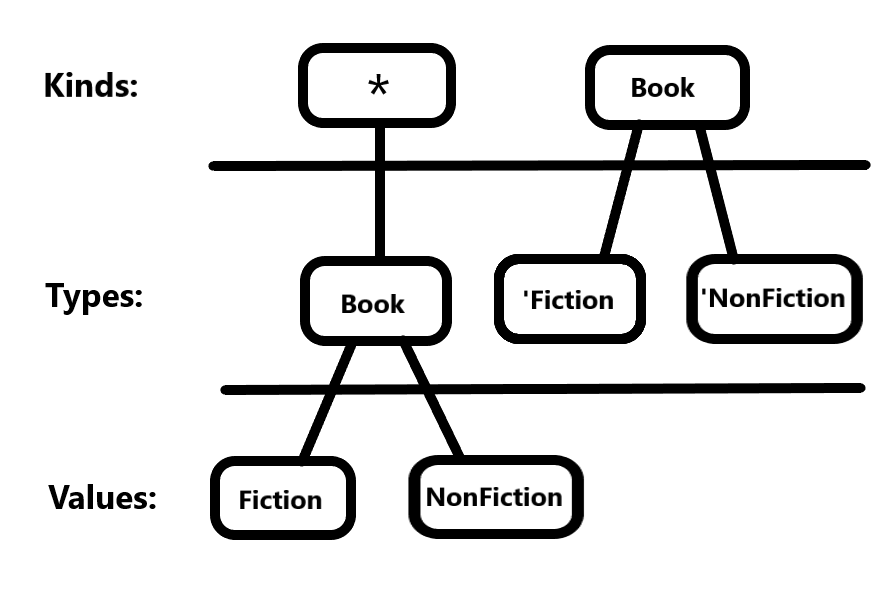
\includegraphics[width=0.8\textwidth,keepaspectratio]{Promotion.png}
    \label{promotiondiagram}
    \caption{A visual representation of the datatype promotion of the \inline{Book} type.}
\end{figure}

The syntax for ``has type'' and ``has kind'' is in both cases \inline{::}, which is unfortunate; however, in the rest of the document, where the distinction is unclear, it shall be made so. Additionally, the prefix \inline{'} for promoted types is optional, and can be left out where the compiler can unambiguously state whether an expression should be a type or a value.

\subsection{Type Families}

Another key extension introduces \emph{type families}~\cite{opentfs,closedtfs}. Type families allow the programmer to compute over types just as functions compute over values; they are the type-level analogue to functions, and come with their own syntax. Following on from the \inline{Book} example above, consider a type family \inline{IsFiction}, which states whether a given \inline{Book} is fiction or not. A value-level definition could be as follows:

\begin{lstlisting}
isFiction :: Book -> Bool
isFiction Fiction    = True
isFiction NonFiction = False
\end{lstlisting}

And the type family analogue is thus, where \inline{::} below means ``has kind'':

\begin{lstlisting}
type family IsFiction (x :: Book) :: Bool where
    IsFiction 'Fiction    = True
    IsFiction 'NonFiction = False
\end{lstlisting}

Both function and family use pattern-matching, and although the type family syntax is a little more verbose, it is still clear. However, the above is a \emph{closed} type family; programmers can define \emph{open} type families which can be extended beyond their initial definition. This mimics ad-hoc polymorphism, in that different implementations of the same type family can be offered with different input kinds.

There are more notable differences between (closed) type families and functions beyond syntax. The most important is that type families cannot be partially applied in the same way that functions can. Consider a function (and closed type family) \inline{IsEitherFiction}, which takes in two books and states whether either of them are fiction or not. A function definition, and a closed type family definition, are below:

\begin{lstlisting}
isEitherFiction :: Book -> Book -> Book
isEitherFiction Fiction _ = True
isEitherFiction NonFiction Fiction = True
isEitherFiction NonFiction NonFiction = False

type family IsEitherFiction (x :: Book) (y :: Book) :: Bool where
    IsEitherFiction 'Fiction _ = True
    IsEitherFiction 'NonFiction 'Fiction = True
    IsEitherFiction 'NonFiction 'NonFiction = False
\end{lstlisting}

While the function \inline{isEitherFiction} can be partially applied, the corresponding type family \inline{IsEitherFiction} cannot. One could feasibly map \inline{isEitherFiction} over a list of books, but mapping with the type family \inline{IsEitherFiction} is impossible. Imagine a type family \inline{Map}, of kind \inline{(a -> b) -> [a] -> [b]}, analogous to the value-level function \inline{map}. While the value-level expression \inline{map (isEitherFiction NonFiction) [NonFiction, Fiction]} evaluates to \inline{[False, True]}, the type-level equivalent (\inline{Map (IsEitherFiction 'NonFiction) '[ 'NonFiction, 'Fiction ]}) causes a type error. Much of functional programming relies on partial application, but these design patterns are impossible when using Haskell's Type Families.

\subsection{First-Class Families} \label{fcfbackground}

The above problem is still an open one in type-level programming, but one solution comes from Li-yao Xia, who put together a Haskell library named First Class Families\footnote{\url{https://github.com/Lysxia/first-class-families}}. First Class Families allow the programmer to map over structures, and specialise type families (\`a la ad-hoc polymorphism), similar to value-level functions. Sadly, First Class Families is not supported by any formal literature on the topic at the time of writing; so we briefly introduce and explain the concept below.

The key idea of this approach is the observation that, while type families cannot be partially applied, type constructors can be. Therefore, by defining type constructors along with a type-level interpreter for them, we can simulate partial type application. It relies on a type, \inline{Exp}, and an open type family, \inline{Eval}. They are defined like so:

\begin{lstlisting}
type Exp a = a -> *
type family Eval (e :: Exp a) :: a
\end{lstlisting}

Passing around the types as \inline{Exp} types allows the programmer to partially apply, and to evaluate whenever they choose with a call to \inline{Eval}. For instance, consider the \inline{IsEitherFiction} type family, but defined in ``First Class Family'' style instead:

\begin{lstlisting}
data IsEitherFiction :: Book -> Book -> Exp Bool
type instance Eval (IsEitherFiction Fiction Fiction) = True
type instance Eval (IsEitherFiction Fiction NonFiction) = True
type instance Eval (IsEitherFiction NonFiction Fiction) = True
type instance Eval (IsEitherFiction NonFiction NonFiction) = False
\end{lstlisting}

We can also define a type-level equivalent of \inline{map} using this technique:

\begin{lstlisting}
data Map :: (a -> Exp b) -> f a -> Exp (f b)
type instance Eval (Map f '[]) = '[]
type instance Eval (Map f (x ': xs))
    = Eval (f x) ': Eval (Map f xs)
\end{lstlisting}

When combined with the above definition of \inline{Map}, mapping (and general Functor behaviour) at the type level becomes possible with the use of \inline{Eval} --- the below expression evaluates to the type \inline{'[ 'False, 'True ]}:

\begin{lstlisting}
Eval (Map (IsEitherFiction 'NonFiction) '[ 'NonFiction, 'Fiction ])   
\end{lstlisting}

Since we use an open type family for the interpreter, there cannot be any overlapping cases as the instances are not ordered. For instance, GHC fails to compile the following definition because \inline{x} could be \inline{'Fiction} or \inline{'NonFiction} and therefore, if \inline{x} were \inline{'Fiction}, either the first or second instance shown below could apply:

\begin{lstlisting}
data IsEitherFiction :: Book -> Book -> Exp Bool
type instance Eval (IsEitherFiction Fiction _) = True
type instance Eval (IsEitherFiction x Fiction) = True
type instance Eval (IsEitherFiction x NonFiction) = False
\end{lstlisting}

When using a closed type family, or a value-level function, the definitions written are implicitly ordered. If instances overlap, the behaviour is to default to the first definition that matches. In Chesskell, we leverage this capability and combine First Class Families with closed type families, where the latter provide the actual implementation of instances of the \inline{Eval} type family. This allows us to have both partial application and the benefits of ordered definitions:

\begin{lstlisting}
data IsEitherFiction :: Book -> Book -> Exp Bool
type instance Eval (IsEitherFiction x y) = IsEitherFiction' x y

type family IsEitherFiction' (x :: Book) (y :: Book) :: Bool where
    IsEitherFiction' 'Fiction _ = True
    IsEitherFiction' x 'Fiction = True
    IsEitherFiction' x 'NonFiction = False
\end{lstlisting}

As part of the development of Chesskell, we have re-implemented many functions from Haskell's standard library using the First Class Family technique. If a First Class Family in the following sections has the same name as a function from Haskell standard library, the reader may assume that the First Class Family has similar behaviour as the value-level equivalent, unless explicitly stated otherwise.

\subsection{Type Applications}

The \inline{-XTypeApplications} Haskell syntax provides a way for the programmer to directly specify type variables~\cite{typeapplication}. Consider an empty list, with type \inline{[a]}. Using type application syntax, where we prefix a type name with \inline{@}, one can specify the type of an empty list by stating what type should inhabit type variable \inline{a}.

For example: the empty list \inline{[] @Int} has type \inline{[Int]}, and the empty list \inline{[] @Bool} has type \inline{[Bool]}. Note that the empty list value has been used in both cases; the thing that has changed is the type of that empty list.

\subsection{Proxies and Singletons}

While promotion and type families allow the programmer to compute at the type level, there must be some way to share information between the value level and the type level for this to be useful. For Chesskell, this communication only needs to be one-way; the value-level EDSL passes information up to the type system, which either compiles successfully or throws a type error. Promoted types (such as \inline{'Fiction}) have no runtime values, and so cannot be used as value-level function argument types. There are two widely used methods of circumventing this limitation in Haskell to mimic values with these promoted types; \emph{proxies} and \emph{singletons}.

\subsubsection{Proxy Types}

Proxy types provide a wrapper to allow arbitrary types to have kind \inline{*}. As we explain above, all value-level functions take in values, and all values have types with kind \inline{*}. The \inline{Proxy} type constructor takes in a single type variable, and exposes a polymorphic value \inline{Proxy}. The \inline{Proxy} type constructor, when applied to some type, has kind \inline{*}. To follow on from the previous \inline{Book} example, while \inline{'NonFiction} has kind \inline{Book}, \inline{Proxy 'NonFiction} has kind \inline{*}, and so a \inline{Proxy} value of type \inline{Proxy 'NonFiction} can be used in value level function definitions. Using the type application syntax we explain above, we can pass around type variables with arbitrary kinds using \inline{Proxy} values.

\subsubsection{Singletons}

As helpful as proxy types can be, they have one limitation; since all the value-level code sees are \inline{Proxy} values, all the relevant information is only available at the type-level. However, singleton types~\cite{singletons} provide an alternative approach. Each singleton type has a single inhabitant value, and each individual value has a single unambiguous type. The types are mirrored in the terms, allowing similar behaviour to dependent types.

This is achieved through, for each defined type, running it through the \textit{singletons} library's Template Haskell definitions\footnote{\url{https://hackage.haskell.org/package/singletons}}. Template Haskell is a compile-time meta-programming system, similar to macros in that it allows programmers to define programs to modify and generate Haskell source code~\cite{templatehaskell}. The singletons library uses Template Haskell to define new data types, given data type definitions. Should \textit{singletons} be given the definition of the \inline{Book} data type which we detail in \cref{promotionsection}, it will generate a new \inline{SBook} data type, defined as below:

\begin{lstlisting}
data SBook :: Book -> * where
    SFiction    :: SBook 'Fiction
    SNonFiction :: SBook 'NonFiction
\end{lstlisting}

Due to data type promotion, this introduces new values, types, and kinds. The runtime value \inline{SFiction} has the type \inline{SBook 'Fiction}, and the type \inline{'SFiction} has kind \inline{SBook Fiction}. These definitions are designed to enable the programmer to access type information through values, and vice versa.

The type of \inline{SNonFiction} can only be \inline{SBook 'NonFiction}, and so value-level code now has some intuition of types; and conversely, when given a type \inline{SBook a}, type families can use the type variable \inline{a} which will be either \inline{'Fiction} or \inline{'NonFiction}.

Chesskell does not make use of singletons; since the Chess rule checking is all done at the type level, there is no need to mirror the types in the values.
\chapter{Design}

In this chapter, we detail the general design of Chesskell. Broadly, Chesskell is split into two main sections; the type-level chess model (which includes the ruleset), and the value-level EDSL which acts as an interface for the type-level chess model.

Additionally, we explain some basic Chess knowledge in this chapter, to aid in understanding. However, we tackle the more complex rules when they become relevant; this chapter does not constitute a formal introduction to Chess, but a simple summary to clarify the design of Chesskell.

\section{The Basics of Chess}

Chess is a two-player game, played in alternating moves by teams typically named \emph{Black} and \emph{White}, after the colours of their pieces. In each turn, the player will move a single piece, and cannot abstain from making a move (or move a piece from its position to that same position). Each piece is governed by its own movement rules, which depend on the state of the board and, in some cases, the history of that piece or other pieces' movements.

\begin{figure}[h]
    \centering
    \fenboard{8/8/8/8/8/8/8/8 w - - 0 1}
    \showboard
    \caption{An empty chess board.}
    \label{chessboard}
\end{figure}

\subsection{The Board}

The board is an 8x8 grid of 64 square tiles, each of which is coloured Black or White such that each square is next to tiles of the opposite colour (see \cref{chessboard}). The pieces move within this board, and cannot take moves that would wrap around it or take them off of the board.

At the beginning of the game, all Chess pieces lie in a specific arrangement (see \cref{startboard}). All Black and all White pieces are opposite one another, such that their positions are mirrored.

\begin{figure}[h]
    \centering
    \newgame
    \showboard
    \caption{An standard chess board where all pieces are in their starting position.}
    \label{startboard}
\end{figure}

\subsection{The Pieces}

While each team has 16 pieces total, there are only 6 types of pieces; Pawns, Rooks, Knights, Bishops, Queens, and Kings (in rough order of value during play). Each have their own strict movement rules, and in all but a single case, pieces of the opposite team can be \emph{captured} by moving to their square. A capture removes a piece from play; there is no way to regain a piece once captured (although there is a way to transform a Pawn into another piece). We give an example of capturing in \cref{capture}.

\begin{figure}[h]
    \centering
    \fenboard{8/8/2Q5/8/4p3/8/8/8 w - - 0 1}
    \showboard
    \quad
    \hidemoves{1.Qe4}
    \showboard
    \caption{The White Queen captures a Black Pawn by moving to its position, and removing it from play.}
    \label{capture}
\end{figure}

\subsection{The Game}

A King is in \emph{check} when they are in the attack path of another piece. The objective of the game is to place the opponent's King into \emph{checkmate}, whereby every move the King could make is to a position where they would be in check (see \cref{checkmate} for an example). Additionally, a move by a team that would place that team's King into check is an invalid move, and cannot be made.

There are additional ways in which a Chess game may end, such as when two opponents agree to a draw; however, these additional rules concern the players of Chess rather than the game itself, and so are not a part of the implementation of Chesskell.

\begin{figure}[h]
    \centering
    \fenboard{8/8/8/8/8/4Q3/8/R3k3 w - - 0 1}
    \showboard
    \caption{The White Queen and White Rook place the Black King into checkmate.}
    \label{checkmate}
\end{figure}

\subsection{Chess Notation} \label{fensection}

There are two main categories of chess notation; those concerning the state of the game, and those concerning the state of the board. Further relevant details on specific Chess notation will be tackled as and when relevant; this section is only aimed as a minor note of their existence.

Chess notation concerning the state of the game tends to be an account of the whole set of moves, starting from the standard start positions. Algebraic notation is the most common chess notation, and is used by FIDE to record matches between professional chess players. Each piece type other than Pawn is denoted with a capital letter: K for King, Q for Queen, B for Bishop, R for Rook, and N for Knight. As such, the move \texttt{Na4} means that a Knight has moved to the position "a4" on the board. Algebraic notation typically does not include the square the piece moved from; only its destination square. \cref{algebraicexample} shows the initial state of the board, followed by a series of moves described with algebraic notation, and the resulting state of the board.

\begin{figure}[h]
    \centering
    \newgame
    \hidemoves{1.e4 e5 2. Nf3 Nc6 3.Bb5 a6}
    \showboard
    \caption{The position of the board after: 1.e4 e5 2. Nf3 Nc6 3.Bb5 a6}
    \label{algebraicexample}
\end{figure}

There are stylised variants of Algebraic Notation, such as Figurine Algebraic Notation, in which symbols for the pieces replace the capital letter. For example, \texttt{Na4} is written as \wmove{Na4}, whereby the N is replaced with the symbol for a Knight. We use Figurine Algebraic Notation, where chess symbols replace capital letters, within this dissertation.

The other class of chess notation is that for board creation or description. Forsyth-Edwards Notation (FEN), a popular example, simply states which pieces are where on a board, line-by-line. White pieces are denoted with uppercase letters, and Black pieces are denoted with lowercase letters. The letters used match those for Algebraic Notation, save for the introduction of P for White Pawns (and p for Black Pawns). Lines are described as series of pieces and empty spaces, such that a row with a White Pawn on every other position would be described as \texttt{P1P1P1P1}. Another row with two spaces between Black Pawns would be described as \texttt{p2p2p1}, since the total number of row positions must equal eight. See \cref{fenexample} for an example of a board created with FEN notation.

\begin{figure}[h]
    \centering
    \fenboard{rnbqkbnr/pppppppp/8/8/4P3/8/PPPP1PPP/RNBQKBNR b - - 0 1}
    \showboard
    \caption{The board created with: (rnbqkbnr/pppppppp/8/8/4P3/8/\\PPPP1PPP/RNBQKBNR b KQkq e3 0 1)}
    \label{fenexample}
\end{figure}

\section{Type-Level Data Structures}

As helpful as type families and First Class Families are in enabling computation at the type level, this computation is useless without something to compute on. Chesskell requires some central repository of information for the state of the board, as well as general data structures for passing around information while validating the Chess ruleset. This section describes the type-level data structures in Chesskell.

\subsection{Chess Data Structures}

An important part of any good Chess program is its board representation, since all other parts of the program come from this; move generation, move evaluation, and the entire search space are all defined or influenced by the board representation. A great deal of work has gone into defining memory- or time-efficient Chess boards~\cite{bitboard,searchtables}, including combinations of multiple representations to yield greater speed~\cite{bitandccr}. While there is value to be gleaned from examining these representations, Chesskell serves a different purpose; it does not need to search through the valid set of moves to determine which are the best, and speed is not its focus. Chesskell's board representation must be relatively efficient, but it would be naive to expect similar levels of performance from type-level constraint solving computation as from optimised value-level code.

\subsection{Singly-linked Lists}

In Chesskell, Haskell's built-in type-level lists are not used as the primary board type. These lists are singly linked, and so have a variable length which can be queried in $O(n)$ time. Ensuring that the chess board remains an 8x8 grid at all times would incur a repeated cost on the compile time of the program, whereby it is checked every time it is used. However, these lists are used for data which can be of variable length; such as the list of available moves for a piece in a specific position.

\subsection{Finger Trees}

An alternative to type-level lists would be to use 2-3 Finger Trees~\cite{fingertrees}. Unfortunately, singly-linked lists have no quick "append" operation. As such, combining lists of moves takes $O(n)$ time, which could be considerable for pieces like Queens who have many moves available to them at any one time. However, Finger Trees can be combined in $O(log(min(n_{1}, n_{2})))$ time, where $n_{1}$ and $n_{2}$ are the sizes of the respective FingerTrees. Singly linked lists have an $O(1)$ append, while Finger Trees have an \emph{amortized} $O(1)$ append operation.

Finger Trees are so named because while the main portion of the data is in recursive tree form, each tree maintains two "hands" full of data. Essentially, each of these appendages is a small overflow buffer for the tree itself, since inserting into the tree is more costly ($O(log n))$) than inserting into the buffer ($O(1)$). A useful side effect of this approach is that not only can you access data at the beginning of the sequence in $O(1)$ time, but you can also access data at the end of the sequence in $O(1)$ time; something impossible with Haskell's built in singly linked lists.

There exists an implementation of Chesskell using Finger Trees as opposed to lists for variable length data, but as we discuss in \cref{fingertreesection}, there was no significant increase in compile time relative to the effort spent implementing Finger Trees at the type level.

\subsection{Length-indexed Vectors} \label{lengthindexedvectors}

If the intention is to use it for representing a Chess board (or any other structure with a definite length), singly-linked lists have issues; how can we ensure that the chess board is the appropriate size (an 8x8 grid) without a length check each move? This would take at least 56 additions, since list length is computed recursively; as well as 7 more addition operations to put together the list lengths.

A more desirable data structure would be one that had a fixed type, which could be guaranteed to remain at length 8. As such, Chesskell makes use of a variant of singly-linked lists, named length-indexed vectors. A length-indexed vector is a singly linked list which contains its' length in its' type. That is, a length-indexed vector of size 0 has a different type than a length-indexed vector of size 3. As with most things in Haskell, we use recursive definitions; an empty vector has length 0, and you express a vector of length (n + 1) by pushing an element to the front of a vector of length n. We give an example GADT data type definition below:

\begin{lstlisting}
data Vec (n :: Nat) (a :: *) where
    VEnd   :: Vec 0 a
    (:->)  :: a -> Vec n a -> Vec (n + 1) a
\end{lstlisting}

If the programmer should require the input vector to be of length 5, then all they must do is include its length in the function definition:

\begin{lstlisting}
someFunc :: Vec 5 a -> b
someFunc vec = -- ...
\end{lstlisting}

This makes it a perfect candidate to act as the central chess board type, containing all pieces. To guarantee that a board is an 8x8 grid, it simply needs to contain 8 length-indexed vectors of length 8. Due to the use of the \inline{-XDataKinds} extension to enable promotion, this length-indexed vector definition immediately also defines a type-level length-indexed vector.

Almost all operations available on lists are available on length indexed vectors. However, since length-indexed vectors have an additional type variable (their length), they are difficult to dynamically create without some length type variable. That is, a function \inline{f :: a -> Vec n b} cannot exist, since the type variable \inline{n} will have nothing to unify with when \inline{f} is called.

\subsection{Type-Level Bitboards}

One popular Chess board representation is the Bitboard~\cite{bitboard}; using a set of 64-bit binary strings to represent the positions of pieces. Since a chess board is always 8x8, a 64-bit string (when seen as a string of 8 bytes) can hold some binary state of a particular Chess board position. Each piece type and colour needs its own bitboard, since a 1 or a 0 is not enough to differentiate between piece types. For instance, a bitboard describing White Pawns will have a 1 at every index in the 64-bit string that has a Pawn present, and will have 0s in all other positions, where the bottom left of the board is the least significant bit, and the top right of the board is the most significant bit.

The main draw of bitboards is the speed at which potential moves can be generated and the board can be modified. For instance, to move all pieces left by one square, all that is required is a left shift by 1 of the bitboard representation. We discuss the topic in more detail in \cref{bitboardconclusion}, and explain why they are not implemented in Chesskell.

% Although type-level Haskell has no bitwise operators, they could potentially be emulated through the use of pattern matching. Consider "bitwise" logical AND; each possible pair of inputs could be pattern-matched against, and the outputs enumerated. However, this code would be both laborious to write and harder to read; and a bitboard representation's main benefit is speed. Type-level operations like this would definitely not map directly to hardware bitwise operations, and so the main benefit of Bitboards would be lost. A Bitboard representation of Chesskell may indeed be faster than the vector board representation we explain above; however, it would incur a considerable complexity cost that is unlikely to be worth it, especially since type-level computation will be slow anyway. While it would make an interesting extension to Chesskell someday in the future, it is not part of the final feature set described in this dissertation.

\section{Modelling Chess with Functions} \label{chesswithfunctions}

Ideally, the Chess board alone would be sufficient to calculate whether a move was valid. A value-level function for determining the validity of moves could take in the current state of the board, and two positions (the position moving from and the position moving two), and either return the new board state or some king of error. Since Chess is conducted move by move, to simulate a game, this function could be chained repeatedly, with each new move and the previous generated board as input. Such an ideal function could have type \inline{ChessBoard -> Position -> Position -> Maybe ChessBoard}.

In a game of Chess, the majority of moves are time-agnostic; that is, they are not tied to previous moves, only the current state of the board. There are, however, two exceptions; Castling and \emph{en passant} capture. Castling is a move by both a King and a Rook, and an \emph{en passant} capture is a special form of capture available only to Pawns. However, the only additional information required to calculate whether these moves are valid is the last piece that moved, and for each piece the number of times that piece has moved. We can extend the board representation to include this information; ensuring that not only pieces and teams are recorded, but also the number of moves made and the last piece to make a move. Therefore, with a new type \inline{DecoratedChessBoard} containing the new information (as well as the board state), a function for calculating move validity could have type \inline{DecoratedChessBoard -> Position -> Position -> Maybe DecoratedChessBoard}.

A pure function implementation is therefore possible, making use of a Chess board data structure which includes this information. Translating this approach to the type-level, we can define a Type Family (or First Class Family) with similar behaviour, of kind \inline{'DecoratedChessBoard -> 'Position -> 'Position -> 'DecoratedChessBoard}. This type-level model of Chess, implemented as a single movement Type Family, must be interacted with via the defined EDSL. The EDSL is responsible for gathering move-wise positional information, and chaining together calls of the movement Type Family, which will either return a valid Chess board or a type error depending on whether the described move is permissible or not.

\subsection{Checking Chess Rules} \label{chessrules}

When determining if a given move of Chess is valid or not, the destination squares for all pieces is not sufficient. In other words, a function to generate the valid positions a piece can move to is not enough to enforce all rules of Chess.

Part of the relevant global state for a Chess game is the team that is currently moving; remember, White and Black teams move in an alternating fashion. It breaks the rules of Chess for a White piece to move after a White piece has just moved. There are also a few implicit Chess rules that would be helpful to have more personalised error messages for; such as the fact that no piece can actually take the opposite King. While this information will be encoded in the fact that the opposite King's position will not be in the valid move list for that piece (even though the piece can indeed attack that position), it would be helpful to have a more specific error message for this case. Instead of \inline{error: The Piece cannot move to that position}, it should say something like \inline{error: Pieces cannot take their King}.

In Chesskell, an early idea was to simply check for these invariants with either type-level if statements or pattern matching. However, as the number of invariants with specific error messages grows, so too would the number of nested if statements. While such an approach would work, it is harder to follow and rather ugly.

Being in a functional environment, it is natural to express these rule checks as functions that either successfully compute something, or return a type error. Each function could essentially act as an assertion; either the input fulfils some query, or there is an error. For instance, a function \inline{CannotTakeKing :: DecoratedChessBoard -> Position -> DecoratedChessBoard} that takes in the board state and the position to move to, and generates a type error if the position to move to is the position of either of the Kings. The reason it returns a \inline{DecoratedChessBoard} in the successful case is so that it can be naturally composed together with the core movement function, using a First Class Family version of the Haskell function composition operator, \inline{(.)}. Instead of code of the form \inline{(if firstCondition then (if secondCondition then Move a1 a2 else throw "Second error") else throw "First error")}, with more and more nested if conditions, the rule-checking code has the form \inline{(SecondCheck . FirstCheck . Move a1 a2)}, which is much easier to modify and understand.

\section{Designing an EDSL for Chess}

Since the EDSL is for describing games of Chess, it makes sense that it should draw inspiration from Chess game notation, such as Algebraic Notation (which we explain briefly above). In such notation, the board state is implicit and undescribed; that is, the state of the board must be inferred by the reader from the moves made thus far, assuming that the game started in standard configuration (\cref{startboard}).

One possible match in Haskell for this style is monadic computation. If the board information were stored in a custom monad, then the \emph{bind} operator (written as \inline{>>=)}) could be used to chain together these chess moves, in some way akin to below:

\begin{lstlisting}
game = chessStart
    >>= move e2 e4
    >>= move e7 e5
    >>= -- ...
\end{lstlisting}

However, this approach introduces a few problems. Firstly, the EDSL is more difficult to read for those unfamiliar with Haskell. It immediately would be less an EDSL, and more a set of plain Haskell functions with nice names. Secondly, it is not immediately clear how a monad for the type-level chess board could be defined. It could piggyback off of another defined monad, such as the \inline{Maybe} monad, but this is introducing further complexity for no good reason.

Luckily, there exists an alternative; Continuation Passing Style (CPS). The core idea is value transformation through a series of continuation function applications, until the final continuation function returns a value. Due to the left-to-right composition of functions, CPS results in very readable code, and could be utilised to avoid any Haskell-specific operators and appear as a clear stretch of Chess notation.

Consider the following example of CPS code. We give the definition of two functions, \inline{add} and \inline{to}:

\begin{lstlisting}
add :: Int -> ((Int -> Int) -> m) -> m
add x cont = cont (+ x)

to :: (Int -> Int) -> Int -> Int
to f x = f x
\end{lstlisting}

With the definition of these two functions, the line \inline{add 5 to 7} is well-typed, and evaluates to \inline{12}. This is because \inline{add} takes in a continuation of type \inline{(Int -> Int) -> m}, and returns a value of type \inline{m}. In other words, the continuation (in this case \inline{to} is responsible for the output. Using such a scheme enables Chesskell to be much closer to conventional chess notation than to Haskell code, and avoids wrapping the types in an unrelated monadic context.
\chapter{Implementation} \label{examplegame}

The final version of Chesskell enables us to describe games of chess, move-by-move. For example, we express a simple 3-move checkmate by the White team as follows:

\begin{lstlisting}
game = chess
    p e4 p f5
    q f3 p g5
    q h5
end
\end{lstlisting}

Note that the spacing is purely for style reasons; the above game could also be written as:

\begin{lstlisting}
game = chess p e4 p f5 q f3 p g5 q h5 end
\end{lstlisting}

\begin{figure}
    \centering
    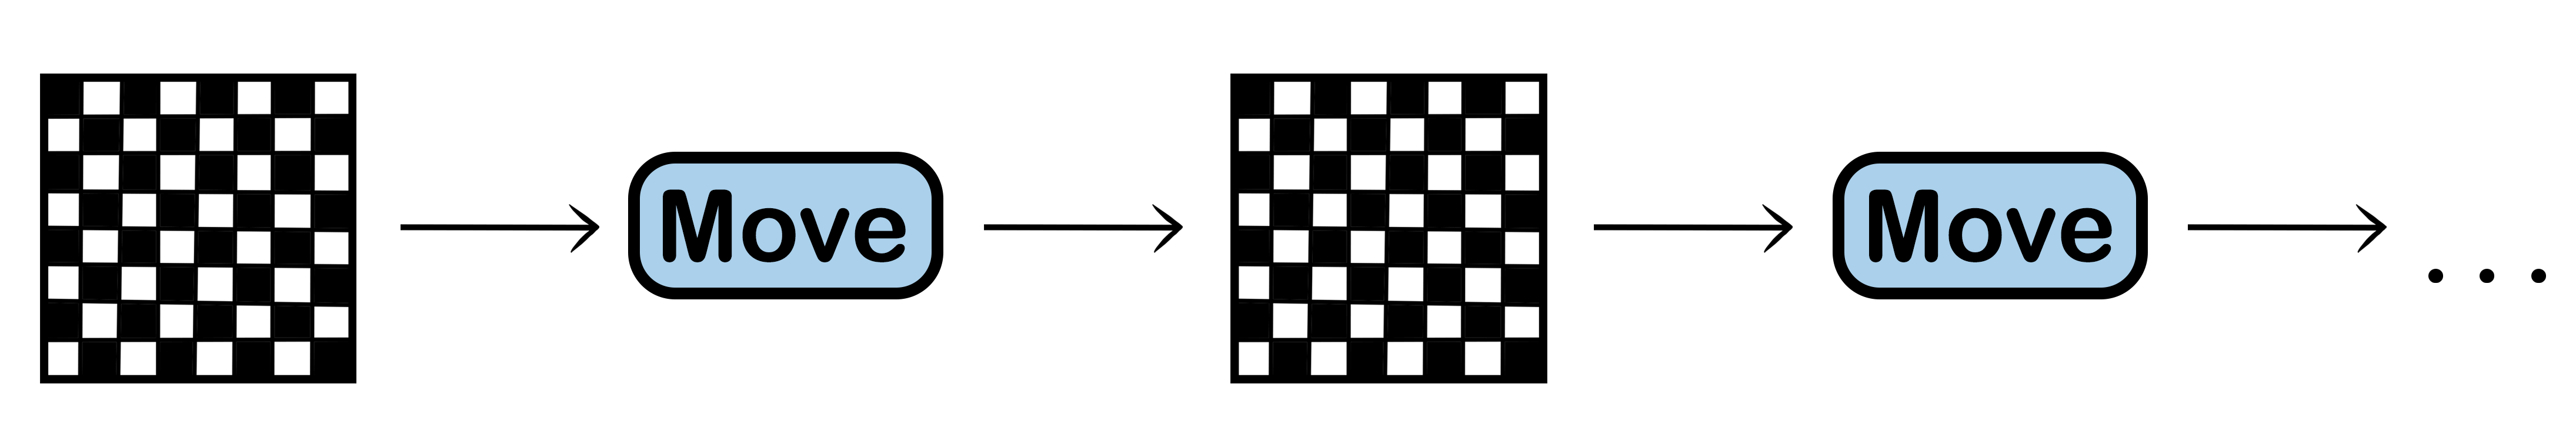
\includegraphics[width=\textwidth,keepaspectratio]{Movefigure.png}
    \caption{A figure demonstrating the chaining of \inline{Move} calls, with each output \inline{BoardDecorator} passed into the next call.}
    \label{movefigure}
\end{figure}

Each move in the Chess game is described with a type family, which takes as input the current state of the board, and outputs the board after the move has been processed (in line with the approach we describe in \cref{chesswithfunctions}). The core movement First Class Family, aptly named \inline{Move}, takes in the position to move from, the position to move to, and the current state of the board, using this information to return a new board state in which the move has been made. Additionally, it updates relevant piece information for the pieces that have moved, which we further detail in this chapter. We give a graphical representation of the process in \cref{movefigure}, and the First Class Family data type for \inline{Move} below:

\begin{lstlisting}
data Move :: Position -> Position -> BoardDecorator -> Exp BoardDecorator
\end{lstlisting}

The EDSL, as we explain in more detail below, uses this \inline{Move} function to perform type-level rule checking of the described Chess game. While the continuation-passing style (CPS) structure complicates the relevant types, the intuition of the EDSL is to take in the current board state, as well as the positions to move from and to, and output the new board state generated by that move. A simplified non-CPS example is below, to aid understanding:

\begin{lstlisting}
edslMove :: Proxy (from :: Position)
         -> Proxy (to :: Position)
         -> Proxy (b :: Board)
         -> Proxy (Eval (Move from to b))
edslMove (x :: Proxy from) (y :: Proxy to) (z :: Proxy (b :: Board))
    = Proxy @(Eval (Move from to b))
\end{lstlisting}

\section{First Class Family Prelude}

In \cref{fcfbackground}, we detail how First Class Families can be utilised to mimic common value-level functions at the type level. While developing Chesskell, we implemented many customary type classes in a First Class Family manner, enabling the final code to be closer to idiomatic Haskell than initially expected.

As an example, consider the \inline{Foldable} typeclass\footnote{\url{https://hackage.haskell.org/package/base-4.15.0.0/docs/Data-Foldable.html}}, which enables value-level data structures with defined \inline{foldr} or \inline{foldMap} instances to be used with many functions written for \inline{Foldable} structures. The type for \inline{foldr} is as follows:

\begin{lstlisting}
foldr :: Foldable t => (a -> b -> b) -> b -> t a -> b
\end{lstlisting}

A value-level function to compute the sum of entries in any foldable collection of integers could be written as such, allowing this definition to be used with any value of a type which implements \inline{Foldable}:

\begin{lstlisting}
sum :: Foldable f => f Int -> Int
sum xs = foldr (+) 0 xs
\end{lstlisting}

In Chesskell, we can express similar behaviour through the use of a new data type, \inline{Foldr}, which we give below with an \inline{Eval} instance for lists:

\begin{lstlisting}
data Foldr :: (a -> b -> Exp b) -> b -> f a -> Exp b
type instance Eval (Foldr f z '[])       = z
type instance Eval (Foldr f z (x ': xs))
    = Eval (f x (Eval (Foldr f z xs)))
\end{lstlisting}

Now, type-level versions of common \inline{Foldable} functions, such as \inline{sum} and \inline{length}, can be implemented using this definition of \inline{Foldr}. We give a type-level First Class Family definition of \inline{Sum} below, along with a simple First Class Family version of natural number addition:

\begin{lstlisting}
data Sum :: f Nat -> Nat
type instance Eval (Sum xs) = Foldr (:+) Z xs

data (:+) :: Nat -> Nat -> Exp Nat
type instance Eval (x :+ y) = x + y
\end{lstlisting}

Mimicking type classes in this manner allows us to implement behaviour akin to Monads and Applicative Functors~\cite{applicatives}. There are certain rules in Chess that would require excessive amounts of pattern-matching to express with closed type families, prompting this effort. In addition to Foldr, Chesskell also includes First Class Family versions of FMap \inline{(<\$>)}, Apply \inline{<*>}, and Bind \inline{(>>=)} (among others), to enable Functor, Applicative Functor, and Monadic behaviour at the type level. We give the definitions of \inline{Bind} and \inline{(>>=)} below, with an \inline{Eval} instance for \inline{Maybe} types, to illustrate:

\begin{lstlisting}
data Bind :: m a -> (a -> Exp (m b)) -> Exp (m b)
type instance Eval (Bind Nothing  f)  = Nothing
type instance Eval (Bind (Just x) f)  = Eval (f x)

data (>>=) :: m a -> (a -> Exp (m b)) -> Exp (m b)
type instance Eval (x >>= f) = Eval (Bind x f)
\end{lstlisting}

\section{Type-Level Chess}

The Chesskell library includes a full representation of a game of Chess at the type-level, as we explain below. The model is checked move-by-move, with the current board state (as well as some additional information) carried between moves via a \inline{BoardDecorator} type. This \inline{BoardDecorator} contains all information necessary to encapsulate the current state of a game of chess; in other words, Chesskell does not rely on any global state, and the game state itself is easily modifiable (enabling the development of board creation syntax, which we detail in \cref{boardcreation}).

\subsection{Chess Types and Kinds}

This section details the types involved, including the board representation; we describe Chesskell's types from the bottom up, since the types here are composite and require understanding of other types.

\subsubsection{Team and PieceName}

Both \inline{Team} and \inline{PieceName} are simple algebraic data types, with all constructors defined in code. The \inline{Team} type enumerates all teams a piece can belong to; \inline{Black} and \inline{White}. The \inline{PieceName} type enumerates all possible names of pieces; Pawn, Rook, and so on. Thanks to promotion, as we explain in \cref{promotionsection}, these types are immediately available for use with Type Families.

\begin{lstlisting}
data Team = Black | White
data PieceName = Pawn
               | Bishop
               | Knight
               | Rook
               | King
               | Queen
\end{lstlisting}

\subsubsection{Position}

The \inline{Position} type holds the positions of pieces on the chess board. It makes use of two more types; one for columns and the other for rows (we explain details on columns and rows in \cref{boarddetails}). The \inline{Column} type is another simple algebraic data type enumerating all columns that a piece can reside within. The row type is a type-level implementation of Peano natural numbers, named \inline{Nat}. Early versions of Chesskell had a custom implementation, but the final version uses definitions provided in \inline{Data.Type.Nat}. We give a definition of \inline{Nat} below, for understanding:

\begin{lstlisting}
data Column = A | B | C | D | E | F | G | H
data Nat where
    Z :: Nat
    S :: Nat -> Nat
\end{lstlisting}

Note that the \inline{Position} kind has a potentially infinite number of valid types, but only 64 of these types are valid chess positions. As such, we define an associated type family, \inline{IsValidPosition}, which outputs \inline{True} if the given position is a valid chess position, and \inline{False} otherwise. We give the definition of the \inline{Position} type below:

\begin{lstlisting}
data Position where
    At :: Column -> Nat -> Position
\end{lstlisting}

\subsubsection{The Pieces}

Each piece, represented by the \inline{Piece} type, contains information relevant for rule checking: that piece's team, name, and an information type. The information type, named \inline{PieceInfo}, contains a \inline{Nat} and a \inline{Position}, to represent the number of moves that piece has taken, and its current position on the board (respectively). Recording the number of moves the piece has taken is important for several rules in chess, including castling and \textit{en passant} capture (as we discuss in \cref{castlesection,passantsection}), and so is included in the \inline{PieceInfo} type.

The \inline{PieceInfo} type was created separately from the plain \inline{Piece} type so that if any further information was required, it could be added without breaking existing \inline{Piece} pattern-match definitions.

\begin{lstlisting}
data PieceInfo where
    Info :: Nat -> Position -> PieceInfo

data Piece where
    MkPiece :: Team -> PieceName -> PieceInfo -> Piece
\end{lstlisting}

There are several utility Type Families defined for the \inline{PieceInfo} type to simplify code; such as \inline{GetPosition}, a First Class Family which gets the position information from a given \inline{PieceInfo} type.

\subsubsection{The Board} \label{boardtypesection}

We explain in \cref{lengthindexedvectors} that length-indexed vectors are an ideal choice for representing the Chess board, as Chess boards have a fixed constant size; with length-indexed vectors, we can enforce the length of the vector in its type, ensuring that the Chess board does not change size. Therefore, it is appropriate to express the board as a vector of 8 vectors of 8 \inline{Maybe Piece}-s. We use \inline{Maybe Piece} instead of just \inline{Piece} because a board square does not necessarily contain a piece:

\begin{lstlisting}
type Eight = (S (S (S (S (S (S (S (S Z))))))))
type Row   = Vec Eight (Maybe Piece)
type Board = Vec Eight Row
\end{lstlisting}

Although this is the main board type, it is augmented with a \inline{BoardDecorator}, so named because the intention is similar to the decorator design pattern~\cite{decorator}, with the exception that sub-classing and super-classing are not features of Haskell. In most cases, we use \inline{BoardDecorator} instead of \inline{Board}, since it contains additional information:

\begin{itemize}
    \item The last team to move;
    \item The last position moved to;
    \item The White and Black King positions, stored as a tuple;
    \item The number of moves in the game thus far.
\end{itemize}

Previous versions of the program, to find the King positions (for the frequent operation of determining if either King is in check), would pass repeatedly over the \inline{Board}. Having their positions available in the decorator avoids the performance cost of making these passes. While this approach introduces overhead (the \inline{BoardDecorator} must be updated each move), the code is much conceptually clearer with the use of the decorator. We give the definition of \inline{BoardDecorator} below:

\begin{lstlisting}
data BoardDecorator where
    Dec :: Board
        -> Team
        -> Position
        -> (Position, Position)
        -> Nat
        -> BoardDecorator
\end{lstlisting}

\subsection{Custom Type Errors}

In Chesskell, we use definitions found in \inline{GHC.TypeLits} to express custom type errors. These definitions include a type family, \inline{TypeError}, and a data type \inline{ErrorMessage}, to enable programmers to generate type errors with arbitrary error messages. For instance, the type below (when type-checked) will cause GHC to halt compilation and generate a type error:

\begin{lstlisting}
type ErrTest = TypeError (Text "Custom error!")
\end{lstlisting}

As expected, the generated type error matches the input \inline{ErrorMessage} argument:

\begin{lstlisting}
-- Below results in the following type error:
    -- * Custom error!
    -- * In the type synonym declaration for 'ErrTest'
type ErrTest = TypeError (Text "Custom error!")
\end{lstlisting}

In GHC, the kind returned by \inline{TypeError} is polymorphic; and so the output of a \inline{TypeError} application can be returned from type families with no issues. The book Thinking With Types~\cite{twt} contains a First Class Family equivalent definition, named \inline{TE'}:

\begin{lstlisting}
data TE' :: ErrorMessage -> Exp a
type instance Eval (TE' msg) = TypeError msg
\end{lstlisting}

In Chesskell, we use this definition to return a type error in circumstances where an \inline{Exp a} type is expected (for some type \inline{a}). To illustrate, consider the below definition:

\begin{lstlisting}
type TETest = Eval (If ('True)
    ('Just 5) -- then
    (TE' (Text "Some error"))) -- else
\end{lstlisting}

Assuming that the \inline{If} First Class Family behaves similarly to if-then-else expressions in Haskell, we expect \inline{TETest} to unify with \inline{'Just 5}. This is the case --- it compiles successfully. However, if we pass in a \inline{'False} type instead of a \inline{'True} type as the if condition, the custom type error is thrown:

\begin{lstlisting}
-- Below results in the following type error:
    -- * Some error
    -- * In the type synonym declaration for 'TETest'
type TETest = Eval (If ('False)
    ('Just 5) -- then
    (TE' (Text "Some error"))) -- else
\end{lstlisting}

\subsection{Chess Rules}

In Chesskell, the rules of Chess are expressed as First Class Families that either return a \inline{BoardDecorator} or a type error (as we explain in \cref{chessrules}). Each such rule-check type family has the suffix \inline{-Check}, such as the aptly named \inline{NotTakingKingCheck} and \inline{NotTakingOwnTeamCheck}. These checks are broadly split into pre-move checks, and post-move checks; each check includes a custom error message to make clear to the user where exactly the rule violation occurs.

To illustrate, we give the definition of \inline{NotSamePosCheck}, which checks that the described move is between two distinct positions, and generates a type error otherwise:

\begin{lstlisting}
data NotSamePosCheck :: Position -> Position -> BoardDecorator -> Exp BoardDecorator
type instance Eval (NotSamePosCheck fromPos toPos boardDec)
    = If' (Eval (fromPos :==: toPos))
        (TE' (TL.Text ("Moves from a position to that same position are not allowed.")))
        (ID boardDec)
\end{lstlisting}

We combine and compose rule checks with a First Class Family version of the function composition operator, \inline{(.)}:

\begin{lstlisting}
NotSamePosCheck . ExampleCheck1 . ExampleCheck2
\end{lstlisting}

\subsubsection{Movement Rules}

Each piece's movement is subject to a specific set of rules for that piece. For instance, a King can move a single space in any direction. The \inline{PieceMoveList} First Class Family formalises this, returning a list of spaces that a piece can move to, given that piece as a \inline{Piece} type, and a \inline{BoardDecorator} representing the current state of the board.

\begin{lstlisting}
data PieceMoveList :: Piece -> BoardDecorator -> Exp [Position]
\end{lstlisting}

Consider a \inline{PieceMoveList} instance for Bishops:

\begin{lstlisting}
type instance Eval (PieceMoveList (MkPiece team Bishop info) boardDec)
    = Eval (AllReachableDiag team boardDec (Eval (GetPosition info)))
\end{lstlisting}

Bishops can move diagonally in a straight line by any number of spaces. The type family \inline{AllReachableDiag} is used to get a list of all diagonally ``reachable'' positions. It takes in the \inline{Position} of the relevant piece, that piece's \inline{Team}, and the current state of the board as a \inline{BoardDecorator}. It outputs all diagonal positions that piece can move to.

Reachability for a given direction is defined in Chesskell as all the empty spaces in that direction, stopping at either the first occupied space or the edge of the board. That space is included or excluded depending on whether that space is occupied by a piece of the opposite team, since an attacking piece could move to that space and take the piece there.

We ensure correctness of movement with a pre-move rule-check, named \inline{CanMoveCheck} with kind \inline{Position -> Position -> BoardDecorator -> Exp BoardDecorator}, which checks if there is a piece at the first position that can move to the second position. Additionally, for more specific error messages, there exist a few additional checks, such as \inline{TeamCheck}, which ensures that the same team does not move twice in a row.

The move list, in most cases, prunes all invalid moves for that piece so that any position in the move list for that piece is a valid movement destination. However, there is one important exception: King movement. The move list for a King can include invalid King movement positions, as the move list generation does not check that the King does not move into the attack path of other pieces (i.e. that it doesn't move into check).

This is deliberate, since check is determined on a position-by-position basis, and checking 8 potential positions for check would be expensive. Instead, we make use of a post-move rule-check named \inline{CheckNoCheck} (which we detail in \cref{checksection}) to ensure that neither King moves into check.

\subsubsection{Attack/Capture Rules}

Although they are similar, the list of spaces that a piece can attack and the list of spaces that a piece can move to are not the same. It is neither true that every position a piece can attack is one that it can move to, nor that every position that can be moved to is under attack; for example, pieces can attack the King of the opposite team, but cannot directly move to that King's position and capture it. There are other differences as well, most notably for Pawns and Kings; so \inline{PieceMoveList} cannot be used in general to determine which squares a piece can attack. To address these shortcomings, we define another type family, \inline{PieceAttackList}, which gives the list of all squares that a piece can attack.

\paragraph{Checking for Check} \label{checksection}

One of the most important rules in Chess, that of placing the opposite King in check, cannot be expressed solely through move and attack lists. Any movement can place either King in check, and it is not always the case that a movement by a piece places the opposite King in check; a move may be ruled as invalid because it places that piece's King into check. For instance, if a Black Rook stands between a White Queen and a Black King, the Rook is not allowed to move out of the Queen's attack path, since such a move would put the Black King into check.

However, the only time that check is relevant is after each move. A move by a piece is invalid when it places that piece's King in check, or if it leaves that piece's King in check. We can express this rule with a post-move check, implemented as a First Class Family \inline{CheckNoCheck}.

Early versions of Chesskell naively computed and combined all attack lists for all pieces, and simply checked if the King's position was a member of that combined list. A more efficient approach, found in Chesskell today, is to emulate other pieces' movement code from the King's position.

This approach is based off of the observation that for all pieces except Kings and Pawns, if they can move from position a to position b, then they can also move from b to a. As an illustration, if a Queen at the King's position (of the same team as the King) would be able to reach a Queen of the opposite team, then the King would be in check.

We leverage this behaviour to detect when a King is in check. Several ``rays'' are sent out from the King's position in horizontal, vertical, and diagonal directions (8 in total). These rays detect Queens of the opposite team, as well as Bishops (for diagonal rays) and Rooks (for horizontal and vertical rays). Attacking Pawns are also checked here, for the immediate diagonal positions either above the King (if the King is White) or below the King. If the ray reaches an attacking piece, the ray function returns true; otherwise, it returns false. The ray will immediately stop being cast, and report back with no check possible in that direction (i.e. a \inline{False} type), if a piece of the same team as the King is encountered (since they would block the attack path of a piece of the opposite team).

In addition to the ray approach, we apply Knight movement rules (from the King's position) to check if there are any Knights that could reach the King and place them in check.

There is one last piece type not handled by the above method---Kings. This is deliberate; it would be illegal for a King to move within attacking distance of the opposite King, since then the moving King would be in check.

A code snippet for determining if the King is in check, which checks if any of the above conditions are true, is below for understanding. The First Class Family \inline{Any} returns true if any elements of a list of Booleans are true, and false otherwise. Each of the -\inline{Ray} functions returns true if a piece could place a King in check from that direction, and the \inline{IsKnightAttacking} function returns true if any Knights of the opposite team are reachable from the given position:

\begin{lstlisting}
data IsKingInCheck :: Position
                   -> Team
                   -> BoardDecorator
                   -> Exp Bool
type instance Eval (IsKingInCheck kingPos team boardDec)
    = Eval (Any '[
    SendLeftRay kingPos team boardDec,
    SendRightRay kingPos team boardDec,
    -- ...
    -- Send rays above, below, and in all 4 diagonal directions
    -- ...
    IsKnightAttacking kingPos team boardDec ])
\end{lstlisting}

\subsubsection{Exceptional Rules}

There are a few Chess rules that are dissimilar from all other Chess rules; and implementing these rules requires a different approach from other rule implementations. Since they are of particular interest, the implementation of these rules is detailed here.

\paragraph{Castling} \label{castlesection}

Most Chess rules move a single piece, and can capture another piece to remove it from play. However, the \emph{Castling} move involves the movement of two pieces; the King, and one of their Rooks. Castling can only occur if neither the King nor the Rooks have moved, as long as none of the positions the King would move through are under check, and there are no other pieces between the King and the Rook. It is one of the most complex rules of Chess, and requires many tests before it can proceed.

There are two varieties of Castle; Queen-side Castle and King-side Castle, depending on the direction that the King moves in (either left or right, respectively). Both varieties are shown for the White team in \cref{queensidecastle,kingsidecastle}. Essentially, the King moves either 2 or 3 spaces towards the Rook, and the Rook wraps around to the other side of the King.

In Chesskell, we model castling as a move by the King; valid castling positions are added to the King's move list. A type family, \inline{CanCastle}, is responsible for checking if the King of a certain team can indeed perform castling in either direction, returning a pair of Booleans to state whether the King can castle left or right. The below code snippet illustrates a part of this process:

\begin{lstlisting}
type family CanCastle (t :: Team) (b :: BoardDecorator) :: (Bool, Bool) where
    CanCastle team boardDec = If' (Not' (HasKingMoved team boardDec))
        (ID (CanCastleToEitherRook team boardDec))
        (ID '(False, False))
\end{lstlisting}

The above code first checks if the King has moved; if they have not, then it checks if both Rooks have not moved. If they have not moved either, then it determines if any of the spaces the King would move through are in check, and then if there are any pieces between the King and the Rook. This logical AND chaining is performed using a type family \inline{PairAnd}, which performs element-wise logical AND on ordered pairs of Boolean types.

These checks must pass for the King to be able to castle in that direction; and a pair of Booleans is returned signifying if the King can castle in either direction. For instance, if the King can castle left but not right, then \inline{CanCastle} will return \inline{'(True, False)}.

This extended Castling check illustrates why it is useful to have each piece's move count in the \inline{PieceInfo} type; it enables quickly determining if a King or either of the Rooks have moved. Simply checking if the King or Rooks are in their starting positions is not enough, since they could have just moved back to those positions.

There are no circumstances under which a King is obligated to castle, and so there are no pre- or post-move rule checks. However, a King cannot castle to capture another piece; so these castle positions are not a part of the King's attack list.

\begin{figure}[h]
    \centering
    \fenboard{8/8/8/8/8/8/8/R3K3 w KQkq - 0 1}
    \showboard
    \hidemoves{1. O-O-O}
    \quad
    \showboard
    \caption{A pair of figures, showing a Queen-side Castle involving the White King.}
    \label{queensidecastle}
\end{figure}

\begin{figure}[h]
    \centering
    \fenboard{8/8/8/8/8/8/8/4K2R w KQkq - 0 1}
    \showboard
    \hidemoves{1. O-O}
    \quad
    \showboard
    \caption{A pair of figures, showing a King-side Castle involving the White King.}
    \label{kingsidecastle}
\end{figure}

\paragraph{Pawn Movement and En Passant} \label{passantsection}

Pawns have the most complex movement rules out of any piece, primarily because their attack patterns are different from their movement patterns. Pawns can move one vertical space forwards, but on their first move can move two spaces instead of one. (For a White Pawn, ``forwards'' means towards a row of higher number, and for a Black Pawn, it means towards a row of lower number --- see \cref{pawnfirstmovement}.) However, they cannot capture a piece this way; they can only capture one diagonal space in front of themselves.

\begin{figure}
    \centering
    \fenboard{8/2p5/8/8/8/8/5P2/8 w - - 0 1}
    \chessboard[showmover=false, pgfstyle=cross, color=black, linewidth=0.15em, shortenstart=0.5ex, shortenend=0.5ex, markfields={c5,c6,f3,f4}]
    \caption{A figure demonstrating the positions that a Black and a White Pawn can move to on their first movement.}
    \label{pawnfirstmovement}
\end{figure}

This means that a Pawn can indeed make a diagonal move, but only if there is a capturable piece there. (For instance, a Black Pawn could move downwards diagonally by a single space to capture a White Bishop, but could not move to that square if it were empty or if it were occupied by a White King.) Additionally, Pawns have one more special capture rule; that of \emph{en passant}.

A Pawn can perform an \emph{en passant} capture if a Pawn of the opposite team has moved forwards by two spaces last turn (which can only occur if that was the opposite Pawn's first move), and ended up next to the attacking Pawn. In this situation, the original attacking Pawn can move diagonally to the empty space behind the opposite team's Pawn, capturing it. See \cref{enpassantfigure} for a graphical representation, showing a White Pawn performing \emph{en passant} capture on a Black Pawn.

\begin{figure}
    \centering
    \fenboard{8/2p5/8/3P4/8/8/8/8 b - - 0 1}
    \scalebox{0.7}{\chessboard[showmover=false, pgfstyle=straightmove, arrow=to, linewidth=0.1em, shortenstart=0.5ex, markmoves={c7-c5}]}
    \hidemoves{1... c5}
    \scalebox{0.7}{\chessboard[showmover=false, pgfstyle=straightmove, arrow=to, linewidth=0.1em, shortenstart=0.5ex, markmoves={d5-c6}]}
    \fenboard{8/8/2P5/8/8/8/8/8 b - - 0 1}
    \scalebox{0.7}{\chessboard[showmover=false]}
    \caption{A sequence of three Chess boards, demonstrating an \emph{en passant} capture by White of a Black Pawn.}
    \label{enpassantfigure}
\end{figure}

This capture rule is dependent on several factors; the last move made, as well as the relative positions of the pieces. Furthermore, the capture move does not result in the attacking piece landing on the square of the piece being captured; making it distinct from all other capture rules.

We define a type family, \inline{GetEnPassantPosition}, which is responsible for determining if an \emph{en passant} capture is a valid move for a pawn at a given position:

\begin{lstlisting}
data GetEnPassantPosition :: Position
                          -> BoardDecorator
                          -> Exp [Position]
type instance Eval (GetEnPassantPosition pos boardDec)
    = If'
        (Eval ((GetLastPosition boardDec) `In` Eval (GetLeftRightPositions pos)))  -- condition
    (FromMaybe '[] (EnPassantPosition (GetMovingTeam boardDec) . PiecePosition)
        (Eval (GetPieceAtWhichDec boardDec (GetLastPosition boardDec) (IsPawn .&. PawnMovedTwoLast))))  -- then
        (ID '[])  --else
\end{lstlisting}

First, the type family checks if the position moved to last turn (fetched from the \inline{BoardDecorator} with \inline{GetLastPosition}) is either to the left or the right of the given pawn position. This is the check to determine whether any piece just moved to the left or right of the current Pawn. If this check passes, then there is another check; whether the piece that made that move was a Pawn, and whether it moved two spaces. If that check passes, then the piece's position is fetched and the row is either incremented or decremented (depending on the attacking team) by the type family \inline{EnPassantPosition} to get the single space either above or below that piece --- the target square to perform \emph{en passant} capture.

We use First Class Families to simplify these logical checks. \inline{GetPieceAtWhichDec} returns a \inline{Maybe Piece} depending on whether there is a piece at a given position which fulfils a given predicate, returning \inline{Nothing} if the predicate does not evaluate to true, and the \inline{Just}-wrapped piece otherwise. Additionally, a type-level First Class Family version of \inline{FromMaybe} is used to either transform the \inline{Nothing} type into an empty list \inline{'[]}, or to transform the wrapped value into a singleton list containing the \emph{en passant} capture position.

Implementing \emph{en passant} captures was the driving factor that prompted the creation of the \inline{BoardDecorator} type, since the last position moved to was required as part of the process. Ultimately, \emph{en passant} captures are implemented in Chesskell, as we demonstrate with the successful compilation of the below game:

\begin{lstlisting}
enPassant = chess
    p d4 p a6
    p d5 p e5
    p e6  -- En Passant capture!
end
\end{lstlisting}

\paragraph{Pawn Promotion}

Pawns have one last complex movement rule; that of promotion. When a Pawn makes it to the opposite side of the Board, they must be promoted to another piece type; either a Queen, a Bishop, a Rook, or a Knight. Pawns must be promoted; they cannot opt out of promotion.

Implementing Pawn promotion proved difficult, since the core \inline{Move} family we describe in \cref{examplegame} does not hold enough information to determine what piece type a Pawn should be promoted to. While one potential solution is to hold this information as a \inline{Maybe PieceName} in the \inline{BoardDecorator}, promotion is infrequent and never occurs in many games. Therefore, instead of using the base \inline{Move} First Class Family, we define a new First Class Family called \inline{PromotePawnMove} to be used when promotion is necessary:

\enlargethispage{\baselineskip}  % Avoid widow in listing below

\begin{lstlisting}
data PromotePawnMove :: Position -> Position -> PieceName -> BoardDecorator -> Exp BoardDecorator
type instance Eval (PromotePawnMove fromPos toPos promoteTo boardDec)
    = If' (Eval (IsPieceAtWhichDec boardDec fromPos (IsPiece Pawn)))
        ((PromotePieceTo promoteTo toPos . Move fromPos toPos) boardDec)
        (If (Eval (IsPieceAt boardDec fromPos))
            (TE' (TL.Text ("The piece at: " ++ TypeShow fromPos ++ " is not a " ++ TypeShow Pawn ++ ". Non-Pawn pieces cannot be promoted.")))
            (TE' (TL.Text ("There is no piece at: " ++ TypeShow fromPos ++ "."))))
\end{lstlisting}

\inline{PromotePawnMove} is similar to \inline{Move}, and indeed calls it internally; but in addition to promoting the piece after it has moved, it ensures that the position to be moved from contains a Pawn (since it is the only piece type that can be promoted).

The type family \inline{PromotePieceTo} of kind \inline{PieceName -> Position -> BoardDecorator -> Exp BoardDecorator} is responsible for changing the \inline{PieceName} of the Pawn piece once it has reached the opposite end of the board. It applies a First Class Family, \inline{PromoteTo}, to the piece at the given position to change its \inline{PieceName} to some given one. Additionally, it generates a type error if the user attempts to promote the Pawn to a King or another Pawn.

However, \inline{PromotePieceTo} and \inline{PromotePawnMove} alone are not enough; because a Pawn must always promote when it reaches the opposite end of the board. To enforce this rule, we define a post-move check named \inline{ShouldHavePromotedCheck}, which is responsible for determining whether a promotion should have occurred at the last move or not. The First Class Family definition simply calls a type family:

\begin{lstlisting}
data ShouldHavePromotedCheck :: Position -> BoardDecorator -> Exp BoardDecorator
type instance Eval (ShouldHavePromotedCheck toPos boardDec)
    = ShouldHavePromotedCheck' toPos boardDec
\end{lstlisting}

The \inline{ShouldHavePromotedCheck'} type family takes in the last position moved to, and the post-movement \inline{BoardDecorator}. If the last move was to the top or bottom rows (i.e. the 8th or the 1st), it checks if there is a Pawn at that position. If so, it generates a type error (since such a Pawn should have been promoted). Otherwise, it returns the input \inline{BoardDecorator}. We give part of the definition below, to illustrate:

\begin{lstlisting}
type family ShouldHavePromotedCheck' (t :: Position) (b :: BoardDecorator) :: BoardDecorator where
    -- ...
    ShouldHavePromotedCheck' (At col Nat8) boardDec
        = If'
            (Eval (IsPieceAtWhichDec boardDec (At col Nat8) (IsPawn .&. HasTeam White))) -- condition
                (TE' (TL.Text ("Promotion should have occurred at: " ++ TypeShow (At col Nat8) ++ ". Pawns must be promoted when they reach the opposite end of the board.")))  -- then
            (ID boardDec) -- else
    -- ...
\end{lstlisting}

Pawn promotion is successfully implemented in Chesskell --- if a pawn should fail to promote during a game of Chess, then a descriptive type error is generated:

\begin{lstlisting}
-- Below results in the following type error:
-- error: Promotion should have occurred at: A8. Pawns must be promoted when they reach the opposite end of the board.
failedToPromote = create
    put _Wh _P at a7
startMoves
    p a8
end
\end{lstlisting}

\section{The EDSL}

The EDSL has gone through multiple changes during development, not only in syntax but also in feature set. This section of the dissertation details the changes the Chesskell EDSL has undergone, explaining the design decisions along the way.

\subsection{Minimum Viable Product}

Before the final format and syntax of the EDSL was decided upon, it was important to determine whether the creation of a value-level interface for the type level model was possible at all. The earliest version of the ``EDSL'' was a set of named Haskell functions, to test if the type-level model was usable by value-level functions.

This Minimum Viable Product version does not include any of the more advanced features of the final EDSLs (such as board creation), but successfully allows the user to describe a Chess game move by move. A single core function, named \inline{move}, made use of \inline{Proxy} types and a First Class Family version of bind to move a piece on a board from one position to another:

\begin{lstlisting}
move :: Proxy (from :: Position)
     -> Proxy (to :: Position)
     -> Proxy (b :: Maybe Board)
     -> Proxy (Eval (b >>= Move from to))
move (sFrom :: Proxy from) (sTo :: Proxy to) (pBoard :: Proxy (b :: Maybe Board))
    = Proxy @(Eval (b >>= Move from to))
\end{lstlisting}

Despite its simple nature, \inline{move} alone is sufficient for a user to interact with the type-level model of Chess and describe a game. It is a viable and minimal version of Chesskell --- if not much of an EDSL.

\subsection{Flat Builders}

Once the feasibility of a Chesskell EDSL was proven, the actual format and logic of the EDSL was to be decided upon. A Continuation Passing Style scheme (as we briefly outline in \cref{cpsshortexample}) forms the foundation for the EDSL, with inspiration taken from Dmitrij Szamozvancev's Flat Builders pattern~\cite{mezzo}. The core idea is value transformation through a series of continuation function applications, until the final continuation function returns a value.

The type \inline{Spec t} is the type of functions which take in a continuation to operate on a value of type \inline{t}. For instance, a function with type \inline{Int -> Spec Int} would take in an integer, and then a continuation to operate on that integer.

\begin{lstlisting}
type Spec t = forall m. (t -> m) -> m
\end{lstlisting}

A function with type \inline{Int -> Spec Int} can be represented with \inline{Conv Int Int} --- the \inline{Conv s t} type represents functions which convert a value of type \inline{s} to a value of type \inline{Spec t}.

\begin{lstlisting}
type Conv s t = s -> Spec t
\end{lstlisting}

Finally, the \inline{Term t r} type ends the continuation stream by taking no continuations; instead, we pass in a value of type \inline{t}, returning a value of type \inline{r}. If \inline{t} and \inline{r} are equal, then an implementation would match that of \inline{id}, the identity function.

\begin{lstlisting}
type Term t r = t -> r
\end{lstlisting}

As an illustrative example of how we use these types, consider the implementation of a sentence-like structure for mathematical operations, such as \inline{to 5 add 7 add 9 increment _then _print}, which should return a string version of the final result. We can achieve this using the Flat Builders pattern. We define \inline{to} like so, passing a number into a continuation which performs some computation on the input:

\begin{lstlisting}
to :: Int -> Spec Int
to x cont = cont x
\end{lstlisting}

We define \inline{add} to take in two input numbers, adding them together, and passing the result to an input continuation:

\begin{lstlisting}
add :: Int -> Int -> Spec Int
add x y cont = cont (x + y)
\end{lstlisting}

We define \inline{increment} like so:

\begin{lstlisting}
increment :: Int -> Spec Int
increment x cont = cont (x + 1)
\end{lstlisting}

The continuation \inline{_then} is intended purely to clarify operations, not to perform any new computation:

\begin{lstlisting}
_then :: Int -> Spec Int
_then x cont = cont x
\end{lstlisting}

And finally, we define the \inline{_print} continuation, which enables us to end the continuation stream and return a string:

\begin{lstlisting}
_print :: Term Int String
_print x = show x
\end{lstlisting}

Using all of these continuations, we can verify that the sentence-like expression \inline{to 5 add 7 add 9 increment _then _print} is well-typed and returns \inline{"22"}, a string.

Note that none of these continuations make assumptions about the kinds of operations performed within the next continuation; only that they take in an integer. Adding new operations, such as multiplication or division, is as simple as adding a new continuation which performs this operation. Such an approach is a natural fit for Chesskell, since the various Chess moves can be (relatively) encapsulated, and it becomes straightforward to extend the EDSL (such as the extensions we discuss in \cref{castleextension,numberextension}).

We combine these Flat Builders continuation types with type-level rule checks, to create a Chess EDSL that operates through passing continuations. Using a combination of proxies, kind signatures, and type applications, we enforce type-level rule checking upon the value-level EDSL.

\subsection{Chess Continuations}

In this section, we discuss the rationale behind and definitions created for Chesskell's long-form syntax. For details on the shorthand syntax, see \cref{shorthandexplanation}.

The chess game starts with a \inline{Proxy} value, whose \inline{Proxy} type is parameterised with a \inline{BoardDecorator} type (i.e. the value has type \inline{Proxy BoardDecorator}). We apply continuations, transforming that value, until the chess game ends\footnote{Note that users can still express games which break rules; these games are just not well-typed.}. Chess games begin with the board in a set configuration; and so we define a type \inline{StartDec} of kind \inline{BoardDecorator} to contain all of this information.

\begin{lstlisting}
chess :: Spec (Proxy StartDec)
chess cont = cont (Proxy @StartDec)
\end{lstlisting}

Each core continuation is named after a piece type, such as \inline{pawn} or \inline{king}. All take in a \inline{Proxy (a :: Position)}, a \inline{Proxy} value whose type is parameterised with the relevant \inline{Position} type. We define a new data type, \inline{MoveArgs}, in order to simplify the process of passing information between the continuations; while the \inline{Move} family is a First Class Family, and can be partially applied, it takes in no \inline{PieceName} argument, and so cannot contain all the relevant types which must pass between the continuations.

\begin{lstlisting}
data MoveArgs where
    MA :: BoardDecorator
       -> Position
       -> PieceName
       -> Position
       -> MoveArgs
\end{lstlisting}

We give the definition of the \inline{pawn} continuation below as an example; however, all piece continuations are similar, and only differ in the \inline{PieceName} type passed to the continuation via \inline{MoveArgs}.

\begin{lstlisting}
pawn :: Proxy (b :: BoardDecorator)
     -> Proxy (fromPos :: Position)
     -> Spec (Proxy (MA b fromPos 'Pawn))
pawn (dec :: Proxy b) (from :: Proxy fromPos) cont
    = cont (Proxy @(MA b fromPos Pawn))
\end{lstlisting}

The next continuation, \inline{to}, takes in another \inline{Proxy (a :: Position)} as well as the \lstinline{MoveArgs}, performs the move computation, puts the resulting board decorator into a \inline{Proxy} type, and passes that \inline{Proxy} into the continuation given.

\begin{lstlisting}
to :: Proxy (MA (b :: BoardDecorator) (fromPos :: Position) (n :: PieceName))
   -> Proxy (toPos :: Position)
   -> Spec (Proxy (Eval (MoveWithStateCheck n fromPos toPos b)))
to (args :: Proxy (MA (b :: BoardDecorator) (fromPos :: Position) (n :: PieceName))) (to' :: Proxy toPos) cont
    = cont (Proxy @(Eval (MoveWithStateCheck n fromPos toPos b)))
\end{lstlisting}

The final relevant definition is of \inline{end}, which ends the chess game, as well as the continuation stream. The definition of \inline{end} matches that of the identity function, as it performs no additional computation on the input board, simply returning it:

\begin{lstlisting}
end :: Term (Proxy (b :: BoardDecorator)) (Proxy (b :: BoardDecorator))
end = id
\end{lstlisting}

Using the above continuations, we can lay out a chess game, move by move. Consider the game expressed in the EDSL which we describe in \cref{examplegame}. It compiles successfully; but should we modify the game such that Black attempts to move after checkmate, GHC generates a type error, since no moves by Black will be valid:

\begin{lstlisting}
-- Below results in the following type error:
    -- * The Black King is in check after a Black move. This is not allowed.
    -- * When checking the inferred type
    --     game :: Data.Proxy.Proxy (TypeError ...)
game = chess
    pawn e2 to e4
    pawn f7 to f5
    queen d1 to f3
    pawn g7 to g5
    queen f3 to h5
    pawn g5 to g4
end
\end{lstlisting}

Or, should White attempt an impossible move in the middle of the game, such as moving a Queen through another piece, a different type error will occur:

\begin{lstlisting}
-- Below results in the following type error:
    -- * There is no valid move from D1 to D3.
    -- The Queen at D1 can move to: E2, F3, G4, H5, ...
    -- * When checking the inferred type
    -- game :: Data.Proxy.Proxy (...)
game = chess
    pawn e2 to e4
    pawn f7 to f5
    queen d1 to d3
    pawn g7 to g5
    queen f3 to h5
end
\end{lstlisting}

\subsubsection{Shorthand syntax} \label{shorthandexplanation}

While the above continuations are feature-complete, and allow the user to fully describe a game of Chess, the resulting notation is considerably more lengthy than Algebraic Notation or other comparable chess notations. As such, we introduced a shorthand syntax towards the end of development, to allow more concise description of Chess games. (This is the syntax we demonstrate in \cref{examplegame}.)

Consider the original continuation for moving a Pawn, named \inline{pawn}. To move using \inline{pawn}, both the origin and destination squares are required, as well as the use of the continuation \inline{to}. The new shorthand equivalent is a single letter, \inline{p}, which takes in the destination position (and a continuation) and performs the move immediately; calculating the origin square is left to the type-level model, via a type family \inline{MoveTo}:

\begin{lstlisting}
p :: Proxy (b :: BoardDecorator)
  -> Proxy (toPos :: Position)
  -> Spec (Proxy (MoveTo Pawn toPos b))
p (dec :: Proxy b) (to :: Proxy toPos) cont
    = cont (Proxy @(MoveTo Pawn toPos b))
\end{lstlisting}

\inline{MoveTo} knows the destination square, and knows the \inline{PieceName} of the piece that moves there. As such, it can calculate the origin square for that move using the piece type's movement rules in reverse. (Remember, for all pieces except Pawns and Kings, if the piece can move from a to b, then it can also move from b to a.)

For example, as we show in \cref{bishopmovement}, to determine the potential origin squares for a Bishop moving to destination square c5, the Bishop's movement rules are applied to an empty board to see the squares that the Bishop can move to from c5.

\begin{figure}
    \centering
    \fenboard{8/8/8/2B5/8/8/8/8 w - - 0 1}
    \chessboard[showmover=false, pgfstyle=cross, color=black, linewidth=0.15em, shortenstart=0.5ex, shortenend=0.5ex, markfields={a3,b4,d6,e7,f8,a7,b6,d4,e3,f2,g1}]
    \caption{A figure demonstrating the positions a White Bishop can move to from square c5.}
    \label{bishopmovement}
\end{figure}

Then, this move list is filtered based on whether there is a valid piece in the original \inline{BoardDecorator} of the correct team in any of those squares. If the resulting filtered list has length 1 (i.e. it contains a single piece), then we extract and return the position of that single piece; otherwise, there are either no valid origin squares, or multiple valid origin squares, in which case the longer Chesskell syntax should be used.

\begin{figure}
    \centering
    \fenboard{8/8/3B4/8/1B6/8/8/8 w - - 0 1}
    \showboard
    \caption{A board where two White Bishops can move to c5.}
    \label{twobishops}
\end{figure}

As an example of the latter case, consider the board state in \cref{twobishops}. There are two bishops that could potentially move to square c5, and as such Chesskell will not be able to tell which bishop should move to that location, and will fail to compile with a type error:

\begin{lstlisting}
-- Below results in the following type error:
    -- * There is more than one White Bishop which can move to: C5.
    -- Consider using the long-form Chesskell syntax instead.
    -- * When checking the inferred type
    -- twoBishops :: Data.Proxy.Proxy (...)
twoBishops = create
    put _Wh _B at d6
    put _Wh _B at b4
startMoves
    b c5
end
\end{lstlisting}

Or, consider the opposite case, whereby there are no White Bishops which can move to c5 (such as in the Chess board at the start of the game). Chesskell will fail with a different type error, explaining the issue:

\begin{lstlisting}
-- Below results in the following type error:
    -- * There is no White Bishop which can move to: C5.
    -- Consider using the long-form Chesskell syntax instead.
    -- When checking the inferred type
    -- noBishops :: Data.Proxy.Proxy (...)
noBishops = chess
    b c5
end
\end{lstlisting}

Despite the late introduction of this shorthand syntax, it fits into Chesskell as a form of Chess notation as well as a demonstration of type-level modelling. In fact, as we discuss in \cref{shorthand}, it resulted in unexpected performance improvements.

\subsection{Creating Chess Boards} \label{boardcreation}

While Chesskell was originally intended only to describe complete games of Chess, the fact that Chess games always start in a fixed configuration complicated testing. To test something like Castling or Check required many moves before these game states became possible. We extended Chesskell to include arbitrary board creation syntax, to simplify this process.

Individual pieces can be placed down on the board using the \inline{put} and \inline{at} continuations, which are used in combination with \inline{Proxy}-wrapped piece names, teams, and positions to modify a \inline{BoardDecorator} type wrapped within the \inline{Proxy} type constructor. Placing a Black Pawn on square a4 is done like so: \inline{put _Bl _P at a4}.

These commands are paired with a new start continuation, \inline{create}, which passes a \inline{Proxy JustKingsDec} value to a continuation. \inline{JustKingsDec} is a \inline{BoardDecorator} type where the board only contains the Black and White King in their start positions; nothing else.

We use these continuations to build custom boards, along with utility continuations for purposes such as setting the last position moved to. The below Chesskell snippet describes the board seen in \cref{twobishops}, by placing down two White Bishops:

\begin{lstlisting}
create put _Wh _B at d6 put _Wh _B at b4 end
\end{lstlisting}

\subsubsection{FEN board creation}

However, Chesskell board creation syntax becomes overly lengthy when dealing with the placement of many pieces. FEN board creation syntax (which we detail in \cref{fensection}) is notably more concise, able to express an entire row of pieces in a maximum of eight characters. To achieve more compact board creation notation, we implemented new syntax based on FEN notation.

Just like real FEN notation, this Chesskell variant of FEN notation (henceforth abbreviated to CFEN) specifies the chess board line by line. We define a new data type, named \inline{Fen}, to encapsulate the idea of a row of 8 items. Each type constructor represents some amount of empty spaces in the row (much like the numbers in FEN notation), such that they increase the length of the row by that amount:

\begin{lstlisting}
data Fen (n :: Nat) where
    FF  :: Fen Nat0
    F1  :: Fen n -> Fen (S n)
    F2  :: Fen n -> Fen (S (S n))
    -- ...
    F7  :: Fen n -> Fen (S (S (S (S (S (S (S n)))))))
    F8  :: Fen Nat8
\end{lstlisting}

These definitions do not go beyond 8 empty spaces, since Chess board rows are only 8 spaces long.

To this data type, we also add type constructors for pieces, all of which take up a single space, and so increment the length of the row. We suffix the type constructor with -\inline{w} for White pieces, and with -\inline{b} for Black pieces:

\begin{lstlisting}
data Fen (n :: Nat) where
    -- ...
    Pw  :: Fen n -> Fen (S n)
    Nw  :: Fen n -> Fen (S n)
    -- ...
    Bb  :: Fen n -> Fen (S n)
    Rb  :: Fen n -> Fen (S n)
\end{lstlisting}

\enlargethispage{\baselineskip}  % Avoid widow in paragraph below

This \inline{Fen} type is used to create a type-level stack of elements; for example, \inline{F5 (Nw (Qw (F1 FF)))}. Each of these \inline{Fen} type constructors can be pattern-matched on to create a list (or vector) of items.

The type family \inline{FenToRow} does exactly that; given a type of kind \inline{Fen n}, it outputs a \inline{Vec n (Maybe Piece)}, essentially transforming it into the row of a board. It also takes another \inline{Nat}, so that each piece's position can be set correctly. Below, the type family \inline{FenReverse'} reverses a \inline{Fen} stack. Since stacks are LIFO structures, and we want the input piece types to be placed left-to-right, the stack must be reversed before use:

\begin{lstlisting}
type family FenToRow (f :: Fen Eight) (r :: Nat) :: Row where
    FenToRow x r = FenHelper (FenReverse' x) r A
\end{lstlisting}

The definition of \inline{FenHelper} is lengthy, but it exists to, given some \inline{Fen} stack of length $n$, a natural number, and a column, return a \inline{Vec n (Maybe Piece)} by transforming the stack elements into a vector of pieces. For instance, given an empty stack, it should return a vector of size 0, and given a stack describing 8 empty spaces, it should return a vector of length 8, populated with \inline{Nothing} types:

\begin{lstlisting}
type family FenHelper (f :: Fen n) (r :: Nat) (c :: Column) :: Vec n (Maybe Piece) where
    FenHelper FF row col = VEnd
    FenHelper F8 row col = EmptyRow
    -- ...
\end{lstlisting}

For each type constructor representing $n$ empty spaces, \inline{FenHelper} returns a vector with those empty spaces pushed to the front. Note that the \inline{Column} argument is incremented to the right by the amount of empty spaces --- knowing the exact column being operated on is helpful for giving pieces correct starting positions:

\begin{lstlisting}
type family FenHelper (f :: Fen n) (r :: Nat) (c :: Column) :: Vec n (Maybe Piece) where
    -- ...
    FenHelper (F1 fen) row col
        = Nothing :-> FenHelper fen row (R col)
    FenHelper (F2 fen) row col
        = Nothing :-> Nothing :-> FenHelper fen row (R (R col))
    -- ...
\end{lstlisting}

Finally, for each of the constructors representing a piece, a corresponding piece (of the given team) is pushed to the front of the vector, with its position populated using the given column and row information:

\begin{lstlisting}
type family FenHelper (f :: Fen n) (r :: Nat) (c :: Column) :: Vec n (Maybe Piece) where
    -- ...
    FenHelper (Pw fen) row col
        = Just (MkPiece White Pawn (Info Z (At col row)))
            :-> FenHelper fen row (R col)
    FenHelper (Nw fen) row col
        = Just (MkPiece White Knight (Info Z (At col row)))
            :-> FenHelper fen row (R col)
    -- ...
    FenHelper (Bb fen) row col
        = Just (MkPiece Black Bishop (Info Z (At col row)))
            :-> FenHelper fen row (R col)
    FenHelper (Rb fen) row col
        = Just (MkPiece Black Rook (Info Z (At col row)))
            :-> FenHelper fen row (R col)
\end{lstlisting}

To give the end user a value-level way to create these \inline{Fen} types, we define continuations for each type constructor of \inline{Fen}. We give some example definitions below:

\begin{lstlisting}
fn7 :: (Proxy (b :: Fen n))
    -> Spec (Proxy (F7 b))
fn7 (Proxy :: Proxy (b :: Fen n)) cont
    = cont (Proxy @(F7 b))

fn8 :: Term (Proxy (b :: Fen Nat8)) (Proxy (b :: Fen Nat8))
fn8 = id

wP :: (Proxy (b :: Fen n)) -> Spec (Proxy (Pw b))
wP (Proxy :: Proxy (b :: Fen n)) cont
    = cont (Proxy @(Pw b))
\end{lstlisting}

\inline{fn0} and \inline{ff} are delimiters; their definitions are different as they are intended to bookend each use of these FEN continuations:

\begin{lstlisting}
ff :: Spec (Proxy FF)
ff cont = cont (Proxy @FF)

fn0 :: Term (Proxy (b :: Fen n)) (Proxy (b :: Fen n))
fn0 = id
\end{lstlisting}

Stacks of \inline{Fen} types can now be created like so: \inline{ff fn1 wQ wN fn5 fn0}. Now that users can create these stacks via value-level constructs, we provide functionality to make use of them. Using \inline{FenToRow}, we define a series of continuations for setting each row of the board with CFEN notation. Each continuation has naming convention ``fen-n'', where $n$ is the row being populated: \inline{fen1}, \inline{fen2}, and so on. To illustrate, we give the definition of \inline{fen5} below:

\begin{lstlisting}
fen5 :: (Proxy (b :: BoardDecorator))
     -> (Proxy (f :: Fen Eight))
     -> Spec (Proxy (SetRowDec' b Nat5 (FenToRow f Nat5)))
fen5 (Proxy :: Proxy b) (Proxy :: Proxy f)) cont
    = cont (Proxy @(SetRowDec' b Nat5 (FenToRow f Nat5)))
\end{lstlisting}

Note that these stacks of \inline{Fen} types must be of length 8 (i.e. they must have kind \inline{Fen Eight}) to be accepted by the continuations, ensuring that the user cannot create rows of the wrong size. To put it all together, these commands can be used together to create a board row-by-row. Below is the CFEN notation to create the board seen in \cref{fenexample}, which would be excessively lengthy if using the basic Chesskell board creation notation:

\begin{lstlisting}
fenBoard = create
    fen1 (ff bR bN bB bQ bK bB bN bR fn0)
    fen2 (ff bP bP bP bP bP bP bP bP fn0)
    fen3 (fn8)
    fen4 (fn8)
    fen5 (ff fn4 wP fn3 fn0)
    fen6 (fn8)
    fen7 (ff wP wP wP wP fn1 wP wP wP fn0)
    fen8 (ff wR wN wB wQ wK wB wN wR fn0)
end
\end{lstlisting}
\chapter{Evaluation}

In this chapter, we evaluate Chesskell in the context of both Haskell and other Chess notations. Additionally, we describe the testing process used to ensure Chesskell meets its specification.

\section{Testing} \label{testsection}

One of the priorities during development was a robust testing procedure. We explain below the various methods of testing employed, including details on how these tests were conceived.

\subsection{Type-level Unit Testing} \label{reflsection}

Usually, unit tests exist to model dynamic behaviour; to check whether running code can perform (or fail to perform) specific operations. However, in Chesskell, the runtime behaviour is very minimal, as all Chess rules are enforced statically through the types. One method of unit testing this static behaviour would be to put definitions into a file, and see if they compile; and indeed, some of the Chesskell tests are carried out in this manner (see \cref{gametestsection}). But this method is unwieldy, and using one of Haskell's pre-existing testing frameworks allows quicker testing and a clearer view of the results of the test suite.

One way of dynamically asserting some static behaviour is to use GHC \emph{deferred type errors}~\cite{deferredtypeerrors}, by which type errors occur as runtime exceptions (i.e. as values of type \inline{TypeError}) whenever a value which causes a type error is evaluated. These runtime exceptions can be pattern-matched on, allowing value-level code to check if an exception generated by a given code snippet is a type error.

Two assertions by other authors are used in Chesskell to craft unit tests for types in this manner: \inline{shouldTypecheck}, defined in the Mezzo library\footnote{\url{https://hackage.haskell.org/package/mezzo}}, and \inline{shouldNotTypecheck}, an HSpec library\footnote{\url{https://hackage.haskell.org/package/should-not-typecheck}}. These assertions pass or fail depending on whether a given expression, when evaluated, generates a deferred type error or not.

For instance, \inline{shouldTypecheck (2 == 3)} should pass, since even though \inline{2} is not equal to \inline{3}, checking for equality between two numbers in this manner is well-typed. However, \inline{shouldTypecheck (not 5)} should fail, since the function \inline{not} has type \inline{Bool -> Bool}, and the value \inline{5} cannot have the type \inline{Bool}.

We use Haskell's HSpec library, for behaviour-driven testing~\cite{hspec}, to create many unit tests with which to test the project. Most commonly, we employ these individual unit tests to test the behaviour of individual type families and First Class Families, such as in the example we give below:

\begin{lstlisting}
oppositeTeamTest :: White :~: Eval (OppositeTeam Black)
oppositeTeamTest = Refl
-- ...
shouldTypecheck oppositeTeamTest
\end{lstlisting}

Note the use of the \inline{(:~:)} type in the above test; this type is defined in \inline{Data.Type.Equality}, and is used as a value-level proof of type equality. It has a single value, \inline{Refl}, with type \inline{a :~: a}. In other words, if you define a \inline{Refl} value with the type \inline{t1 :~: t2} for some types \inline{t1} and \inline{t2}, then this definition will only type check if \inline{t1 ~ t2}; that is, if they can unify. Above, we can see this put to use -- the \inline{Refl} value with type \inline{White :~: Eval (OppositeTeam Black)} will produce a type error if the opposite team of Black is not White. We use the \inline{(:~:)} type often in Chesskell unit tests, as it provides a simple way of asserting that two types are equal.

\subsubsection{Scenario Testing} \label{scenariosection}

The behaviour of many of the type families in Chesskell depends on the current board state. As an example, consider Pawn movement; the valid moves for a Pawn vary based on whether it is that Pawn's first move, on the pieces around the Pawn, and on the last move made. To test corner cases, we construct test boards which should bring about specific behaviour in the type families tested, perhaps even causing those type families to generate a type error. During development, this manner of testing was nicknamed "Scenario Testing", and it shall henceforth be referred to as such.

For instance, both team's Kings should always be on the board. To have a King absent from one of the teams should result in undefined behaviour, as such an event signals a clear departure from the rules of Chess. To test this behaviour, we create a unit test on an empty board (which will naturally be missing both Kings), and ensure that failing to find the King of a specific team on that board results in type error:

\begin{lstlisting}
findKingTest :: Proxy (a :: Piece)
findKingTest = Proxy @(Eval (FindKing White EmptyDec))
-- ...
shouldNotTypecheck findKingTest
\end{lstlisting}

Note that the \inline{(:~:)} type we use in \cref{reflsection} is not used here; instead, we define the test with a \inline{Proxy a} type. Since we are expecting the above type variable \inline{a} to fail unification with a type error, there is no need to compare \inline{a} with any other type. We use \inline{Proxy} types rather than \inline{(:~:)} types when equality testing is not required, such as in cases where we expect a test to generate a type error.

For a more involved example of the unit testing process, consider Castling (a Chess move we detail in \cref{castlesection}). There are situations in which a team can castle in one direction, but not in the other direction; and in those situations, calling \inline{CanCastle} for that team should return \inline{True} for the valid direction, and \inline{False} for the invalid one. To test this behaviour, we create a custom Chess board (see \cref{castleboard} for a visual representation) named \inline{CastleDec}, in which the Black King can castle left but not right, and the White King can castle right but not left. We pair this custom board with two unit tests, to ensure that \inline{CanCastle} has the expected behaviour:

\begin{lstlisting}
canCastleBlackTest :: '(True, False) :~: CanCastle Black CastleDec
canCastleBlackTest = Refl

canCastleWhiteTest :: '(False, True) :~: CanCastle White CastleDec
canCastleWhiteTest = Refl
-- ...
shouldTypecheck canCastleBlackTest
shouldTypecheck canCastleWhiteTest
\end{lstlisting}

\begin{figure}
    \centering
    \fenboard{r3k1pr/8/8/8/8/8/8/RP2K2R w - - 0 1}
    \showboard
    \caption{A board where the Black King can castle left but not right, and the White King can castle right but not left.}
    \label{castleboard}
\end{figure}

\subsubsection{FIDE Laws of Chess Unit Tests}

To ensure correctness as far as possible, we create unit and scenario tests for each FIDE Law of Chess which is amenable to testing in this manner. One of the primary aims of Chesskell, as we state in \cref{introobjectives}, was to implement all FIDE laws concerning the game of Chess itself. An appropriate way of determining the success of this objective is to test as many laws of Chess as possible, to ensure that Chesskell's behaviour matches that of the FIDE ruleset.

As an example, consider the FIDE law outlining how Knights move around the board:

\begin{quoting}
    The knight may move to one of the squares nearest to that on which it stands but not on the same rank, file or diagonal.
\end{quoting}

To test this behaviour, we write a total of 16 unit tests. For both teams, eight tests encompassing movement in the four cardinal directions, as well as the four intercardinal ones. This movement is tested on boards which only contain the relevant Knight, and the two Kings (to avoid the "missing King" error we detail in \cref{scenariosection}). While these tests do not inspect every possible target and destination square, they give reasonable assurances that Knights move correctly around the board:

\begin{lstlisting}
whiteCannotGoLeft :: Proxy (a :: BoardDecorator)
whiteCannotGoLeft = Proxy @(Eval (Move (At D Nat5) (At B Nat5) WhiteKnightDec))

whiteCannotGoRight :: Proxy (a :: BoardDecorator)
whiteCannotGoRight = Proxy @(Eval (Move (At D Nat5) (At E Nat5) WhiteKnightDec))

-- ...

blackCannotGoNW :: Proxy (a :: BoardDecorator)
blackCannotGoNW = Proxy @(Eval (Move (At D Nat5) (At B Nat7) BlackKnightDec))

blackCannotGoNE :: Proxy (a :: BoardDecorator)
blackCannotGoNE = Proxy @(Eval (Move (At D Nat5) (At F Nat7) BlackKnightDec))
\end{lstlisting}

None of these tests should type check, as they involve invalid movement; so we use the \inline{shouldNotTypecheck} assertion:

\begin{lstlisting}
shouldNotTypecheck whiteCannotGoLeft
-- ...
shouldNotTypecheck blackCannotGoNE
\end{lstlisting}

\subsection{Chesskell Game Tests} \label{gametestsection}

To test Chesskell EDSL correctness, we use a similar process to the one we lay out in \cref{scenariosection}. We describe specific Chess scenarios (as plain Haskell source definitions) which should display certain behaviour, and manually ensure that the EDSL either compiles, or fails to compile with a specific type error. To illustrate, we give an example below. As we discuss in \cref{promotionsection}, Pawn promotion is mandatory, and it breaks the rules of Chess if a Pawn reaches the opposite end of the board and is not promoted. To test this, we create a custom Chess board and describe a Chess game in which a Pawn should have been promoted, but has not been. We then compile this described game, ensuring that GHC generates the expected type error:

\begin{lstlisting}
-- Below fails with the following type error:
-- * Promotion should have occurred at: h8. Pawns must be promoted when they reach the opposite end of the board.
-- * When checking the inferred type:
--     didntPromote :: Data.Proxy.Proxy (TypeError ...)
didntPromote = create
        put _Wh _P at h7
        put _Bl _P at a2
    startMoves
        pawn h7 to h8
    end
\end{lstlisting}

Additionally, we express the first few moves of a variety of famous Chess games in Chesskell notation, to ensure that Chesskell also compiles error-free Chess games. For instance, the first few moves of 20 famous Gary Kasparov games have been expressed in Chesskell notation and compiled, to test Chesskell's capabilities.

To add to the previous test suite, we replicate some of the games present, while introducing minor errors. For instance, consider the first 10 moves of the famous game between Loop and Deep Gandalf, two Chess AIs, which (as a Haskell source definition) GHC successfully compiles:

\begin{lstlisting}
loopVsGandalf = chess
        p e4 p c5
        n f3 p d6
        p d4 p d4
        n d4 n f6
        n c3 p a6
    end
\end{lstlisting}

With a separate definition, we recreate this game with a subtle error -- move 10 has been modified to ensure that the Pawn's destination square is the same as its origin square, a move disallowed in Chess:

\begin{lstlisting}
loopVsGandalfError = chess
        p e4 p c5
        n f3 p d6
        p d4 p d4
        n d4 n f6
        n c3 p a7  -- Pawn moves to same place!
    end
\end{lstlisting}

As expected, the error-free version compiles, and the erroneous version fails to compile.

\section{Compile Time and Memory Usage} \label{problemsection}

Key observations for us while developing Chesskell have been unpredictable compile-time and memory usage. While the extensions to Haskell's type system as implemented in GHC are very exciting and, as demonstrated, allow us to implement complex rule systems, it is difficult to debug them -- GHC's performance with respect to type-level computation is opaque to developers. In this section we outline the issues we faced, and describe approaches we found to solve or avoid them.

As we explain above in \cref{testsection}, the Chesskell library is accompanied by an extensive test suite, implemented using HSpec behaviour-driven tests~\cite{hspec} and deferrable type errors to test the outputs of type families adhere to the FIDE ruleset. Compiling this test suite causes GHC memory usage to exceed 27 GB. These memory issues are not specific to the tests, and can be reproduced in longer Chesskell games. Due to these issues, Chesskell games are practically limited to 12 moves before GHC crashes and runs out of memory (on all systems tested), although there is no theoretical limit to the number of moves.

Below, when we state that a Chesskell game takes $n$ seconds to compile, we mean that it takes $n$ seconds to compile the Chesskell description of the 1964/65 USSR Championship game between Ratmir Kholmov and David Bronstein. We chose this game as the benchmark for compile-time comparison, though others are also used to test the functionality of Chesskell (as we mention in \cref{gametestsection}).

\subsection{Finger Trees} \label{fingertreesection}

A common operation in Chesskell is creating lists of potential positions (i.e. move lists and attack lists), and combining them with the append \inline{(++)} operator. However, as we mention in \cref{fingertreedesign}, appending singly-linked lists takes $\mathcal{O}(n)$ time. Since this operation is common, we implemented type-level 2-3 Finger trees~\cite{fingertrees} to take advantage of better amortized append:

\begin{lstlisting}
data FingerTree (a :: Type) where
    Empty  :: FingerTree a
    Single :: a -> FingerTree a
    Deep   :: Digit a -> FingerTree (Node a) 
           -> Digit a -> FingerTree a

data Node a = Node2 a a | Node3 a a a
data Digit a = One a | Two a a | Three a a a | Four a a a a
\end{lstlisting}

We define operations to append both to the start and to the end of the tree as type families, denoted as \inline{:<} and \inline{:>} respectively. We give the definition of \inline(:>) below:

\begin{lstlisting}
type family (:>) (n :: FingerTree a) (x :: a) :: FingerTree a where
    Empty                           :> x
        = Single x
    Single y                        :> x
        = Deep (One y) Empty (One x)
    Deep left middle (One y)        :> x
        = Deep left middle (Two y x)
    Deep left middle (Two y z)      :> x
        = Deep left middle (Three y z x)
    Deep left middle (Three y z w)  :> x
        = Deep left middle (Four y z w x)
    Deep left middle (Four y z w a) :> x
        = Deep left (middle :> Node3 y z w) (Two a x)
\end{lstlisting}

Additionally, we show parts of the definition for an append operation, given as an open type family \inline{(++)}:

\begin{lstlisting}
type instance ((Deep leftL leftM leftR) ++ (Deep rightL rightM rightR))
    = Deep leftL (AddTree1Digit leftM (ToNode leftR rightL) rightM) rightR
-- ...

type family AddTree1Digit (t1 :: FingerTree a)
                          (d1 :: Digit a)
                          (t2 :: FingerTree a)
                          :: FingerTree a where
    AddTree1Digit Empty dig rightTree
        = AddDigitLeft dig rightTree
    AddTree1Digit (Single x) dig rightTree
        = x :< AddDigitLeft dig rightTree
    -- ...
    AddTree1Digit (Deep leftL leftM leftR) dig (Deep rightL rightM rightR)
        = Deep leftL (AddTree1Digit leftM (ToNode leftR rightL) rightM) rightR
\end{lstlisting}

We replaced all append and mapping operations over lists with corresponding operations on Finger Trees. To our disappointment, changes were negligible: compile time went down by an average of 5 seconds and memory usage was reduced by an average of 0.5 GB. Although this is an improvement, it again shows that algorithmic complexity is not responsible for the compiler performance we observe.

\subsection{Checking for Check}

One of the most complex parts of Chesskell involves detecting when a King is placed in check. As we explain in \cref{checksection}, an initial na\"ive implementation of testing for check (named \inline{CheckNoCheck}) involved assembling all possible moves by pieces of the opposite team, and checking if the King position was in that list. The pre- and post-move checks were composed together within a single family, along with the actual movement of the pieces themselves, like so:

\begin{lstlisting}
data Move :: Position -> Position
          -> BoardDecorator -> Exp BoardDecorator
type instance Eval (Move fromPos toPos boardDec) = Eval ((
    ShouldHavePromotedCheck toPos . CheckNoCheck .  -- Post-move checks
    MoveNoChecks fromPos toPos .
        CanMoveCheck fromPos toPos .  -- Pre-move checks
        NotTakingKingCheck toPos .
        NotTakingOwnTeamCheck toPos .
        NotSamePosCheck fromPos toPos .
        NotLastToMoveCheck fromPos .
        TeamCheck fromPos) boardDec)
\end{lstlisting}

Removing the \inline{CheckNoCheck} post-move check entirely (from the codebase using the old implementation) reduced memory usage of an 8-move Chesskell game from 22-23GB to 7.5-8GB, and average compile time from 1 minute 37 seconds to 24 seconds, proving that testing for check was a performance bottleneck.

Attempting to optimise the codebase and reduce memory usage as the result of an ``out of memory'' crash, we created the new ray implementation \cref{checksection}. Despite the reduced computation performed by GHC with the new implementation, there was no noticeable decrease in memory usage when compiling Chesskell games -- GHC continued to run out of memory and crash.

However, splitting out the pre-move rule checks and the post-move rule checks into separate type families helped GHC to terminate, no longer running out of memory. The new implementation (which we give below) takes less than 1 minute and 30 seconds to compile, and uses an average of 25GB of memory. We put the pre-move checks into a new \inline{MoveWithPreChecks} family:

\begin{lstlisting}
data MoveWithPreChecks :: Position
                       -> Position
                       -> BoardDecorator
                       -> Exp BoardDecorator
type instance Eval (MoveWithPreChecks fromPos toPos boardDec) = Eval (
    (MoveNoChecks fromPos toPos .
        CanMoveCheck fromPos toPos .
        NotTakingKingCheck toPos .
        NotTakingOwnTeamCheck toPos .
        NotSamePosCheck fromPos toPos .
        NotLastToMoveCheck fromPos .
        TeamCheck fromPos) boardDec)
\end{lstlisting}

However, we leave the post-move checks in the original \inline{Move} family, joining the two with a call to \inline{MoveWithPreChecks}:

\begin{lstlisting}
data Move :: Position
          -> Position
          -> BoardDecorator
          -> Exp BoardDecorator
type instance Eval (Move fromPos toPos boardDec)
    = Eval ((ShouldHavePromotedCheck toPos . CheckNoCheck)
        (Eval (MoveWithPreChecks fromPos toPos boardDec)))
\end{lstlisting}

While the cause for this increase in performance is unknown, we speculate it may be related to the number of type variables that must be unified at a given time. In any case, this example shows that sometimes improvements to algorithmic complexity of type-level programs can make little difference, while simply restructuring the type families can. Therefore, we believe that there is a need for better tooling as part of GHC to understand what causes such spikes in compile time and memory usage.

\subsection{Type Applications vs. Type Signatures}

We observed a difference in behaviour between type signatures and type applications. Initially, we did not define \inline{StartDec} by hand for use in the definition of \inline{chess} and instead pieced it together through a lengthy series of type family applications:
\begin{lstlisting}
type StartDec = MakeDecorator (ExpensiveOperation (...))
\end{lstlisting}
With this initial version of \inline{StartDec} to set up the game, we attempted two definitions of \inline{chess}: one using a type application and the other using a type signature. These definitions, given below, should be equivalent:
\begin{lstlisting}
chess :: Spec (Proxy StartDec)
chess cont = cont (Proxy @StartDec)

chess :: Spec (Proxy StartDec)
chess cont = cont (Proxy :: Proxy StartDec)
\end{lstlisting}
The version of \inline{chess} using a type application compiles without issues, but causes lengthy (sometimes unrecoverable) pauses at runtime when used. Conversely, when compiling the type signature version, GHC either fails to terminate or crashes due to a lack of memory. This difference in behaviour between the definitions is unexpected and resulted in GHC bug report\footnote{\url{https://gitlab.haskell.org/ghc/ghc/-/issues/18902}}. As a work-around, we have written out \inline{StartDec}'s definition in full in the Haskell source file, allowing compilation and usage of either definition with no issues.

\subsection{Descriptive Error Messages}

We intended for Chesskell's type errors to include the number of the move which resulted in a rule violation, to make errors as clear as possible. Ideally, this would result in error messages such as the one below:

\begin{lstlisting}
-- Below results in the following type error:
-- * There is no valid move from E2 to E5.
--   The Pawn at E2 can move to: E3, E4
--   At move: 1
-- * When checking the inferred type
--   game :: Data.Proxy.Proxy (...)
game = chess pawn e2 to e5 end
\end{lstlisting}

However, adding the move number (taken from the current \inline{BoardDecorator}) to Chesskell's error messages in this manner causes spikes in compile time and memory usage: a game consisting of a single erroneous move, such as the above, results in nearly 26GB of memory usage, and takes close to 2 minutes to compile. For reference, the average compile time and memory usage for that single move game are under 20 seconds and 4.5GB respectively.

Taking other information from the \inline{BoardDecorator} type, such as the position of one of the Kings, and putting it into the error message does not result in similar spikes. Due to its effect on compile time and memory usage, Chesskell error messages do not include the move which broke the rule. Instead, we ensure that Chesskell error messages are detailed enough that the user should be able to find the location of the error.

\subsection{Chesskell Shorthand} \label{shorthand}

One of the most dramatic optimisations in terms of compile-time and memory usage was unexpected and accidental: it resulted from the implementation of the shorthand syntax (\cref{shorthandexplanation}).

With the longhand notation, any Chesskell game longer than 10 moves would cause GHC to crash (on the authors' machines). We predicted that the shorthand syntax would degrade performance and reduce this number, since the type-level model of Chess would not only have to perform all of the move checking, but also determine which piece(s) could move to the destination square. However, since it allowed more concise description of Chess games in line with existing Chess notation, we deemed this trade-off acceptable.

We developed a working version of the shorthand syntax, without going through extensive optimisations or performance testing. Despite the greater amount of work required from GHC to compile these short-hand descriptions, there were notable and significant decreases in average compile time and memory usage: with the longhand syntax, compiling a 10-move Chesskell game took an average of 3 minutes and 25GB of memory, and a 12-move Chesskell game would crash every time. With the shorthand syntax, a 10-move Chesskell game compiles in around 1 minute 20 seconds, using 24GB of memory, and a 12-move Chesskell game compiles in an average of 1 minute 50 seconds, using 25GB of memory.

The shorthand syntax allows for us to express games which are longer by 2 moves, and yet incur no additional penalties on compile time or memory usage. We again speculate that the improvement is due to fewer type variables that need to be unified.

\section{Detailed Performance Analysis} \label{performanceanalysis}

As compile-time and memory usage proved to be a prevalent issue, we performed a more rigorous form of performance analysis towards the end of development, comparing how multiple Chess games affected Chesskell in terms of memory usage and compile time.

All of the Chess games mentioned were expressed in Chesskell's shorthand syntax (see \cref{shorthand}), with a variable number of moves: either 6, 8, or 10. For each game, we tabulate the information gathered on compile time and memory usage, both of which were averaged over three runs of each game for each move limit.

The games compared are:

\begin{itemize}
    \item The 1964/65 USSR Championship game between Ratmir Kholmov and David Bronstein (mentioned in \cref{problemsection});
    \item The 1918 "Berlin Four Masters" game between Akiba Rubinstein and Milan Vidmar;
    \item The 2019 Chinese League game between Zeyu Xiang and Yibo Zhou;
    \item The 2004 Calvia Olympiad game between Julio Ernesto Granda Zuniga and Pedro Mascaro March.
\end{itemize}

As we can see in \cref{performancetable}, the results are consistent with previous behaviour; as the number of moves increases, so too does the memory usage and compile time.

% TODO: Write more??

\begin{table}[h]
    \centering
    \label{performancetable}
    \begin{tabular}{l|ll|ll|ll}
                   & \multicolumn{2}{|l|}{6 moves} & \multicolumn{2}{|l|}{8 moves} & \multicolumn{2}{|l}{10 moves}                      \\
                   & GB                            & Mins                          & GB                            & Mins & GB   & Mins \\
        \hline
        Kholmov    & 13.1                          & 1:41                          & 15.2                          & 2:07 & 24.4 & 2:59 \\
        Rubinstein & 12.4                          & 1:27                          & 24.8                          & 3:27 & 25.9 & 6:10 \\
        Xiang      & 13.0                          & 1:31                          & 25.0                          & 3:02 & 25.8 & 4:28 \\
        Zuniga     & 12.9                          & 1:32                          & 15.2                          & 2:05 & 22.8 & 2:48
    \end{tabular}
    \caption{A table displaying the memory usage (in GB) and the compile time (in minutes) for a selection of Chesskell games.}
\end{table}

\section{Chesskell EDSL vs Other Chess Notations}

One of the aims of Chesskell was for the final Chess EDSL to be closer to existing Chess notation than to Haskell syntax. In this section, we lay out how successful Chesskell has been in this regard, with justifications where Chesskell differs from existing notation.

\subsection{Comparison with Algebraic Notation}

Since FIDE uses Algebraic Notation, it was taken as the exemplary Chess notation to aim towards. In this notation, Chess games are described move-by-move, using the destination square and the piece type for each move. A game equivalent to that given in \cref{examplegame} is given below:

\begin{verbatim}
1. e4 f5 2. Qf3 g5 3. Qh5
\end{verbatim}

There are some differences between Algebraic Notation and Chesskell syntax that are immediately apparent. First of all, Chesskell includes pawns as a piece type in their movement (e.g. \inline{p e4}), whereas Algebraic Notation only uses the destination square. Pawns are included as a piece type in Chesskell, as leaving them out would complicate the relevant continuations. While it does increase the character count when expressing the move, it simplifies implementation and improves clarity to include them, so we deem this trade-off acceptable.

Other differences (such as the space between the piece type and destination square, or the move count) are made for similar reasons, and for personal taste. Below, we outline a few of the more interesting differences.

\subsection{Captures}

Capture moves are usually treated as a special case, having their own special notation. For instance, in Algebraic Notation, capture moves include an x character to set them apart from non-capture moves. As an example, consider a Knight moving to the square d4. If the Knight does not capture another piece, then this is expressed as \wmove{Nd4}. However, if the Knight does indeed remove another piece from play, then the move should be written \wmove{Nxd4}.

Chesskell notation does not treat capture moves as a special case. A move, whether capturing or otherwise, is expressed the same way; the above move would be \wmove{n d4}. Interestingly, this makes Chesskell closer to Minimal Algebraic Notation, which also does not include (similar to Chesskell) special notation for Check, En Passant Capture, and Checkmate.

\subsection{Castling} \label{castleextension}

Notations such as Algebraic Notation tend to have specific notation for Castling; since it is a unique move which moves more than one piece, it is a useful signpost for the reader to update their mental model. Castling is expressed in algebraic notation as either \wmove{0-0} or \wmove{0-0-0}, to represent kingside and queenside castling, respectively.

In Chesskell, castling can be expressed as a King movement: such as \inline{k c1}, and requires no special notation. However, some people may prefer a clearer sign that a move is a castle, and so we include castling notation with the help of a single type family: \inline{CastleMove}. This type family takes in a \inline{BoardDecorator}, representing the current state of the board, and a boolean argument, stating whether the castle move is to the left or right. It returns the new state of the board in which the relevant castling move has been made.

For instance, when the boolean argument is \inline{True}, the relevant King is castling to the right. If the last team to move was \inline{Black}, then the currently moving team is \inline{White} -- and so the target castle position must be g1:

\begin{lstlisting}
type family CastleMove (l :: Bool) (b :: BoardDecorator) :: BoardDecorator where
    CastleMove True  (Dec board Black pos kings n) = MoveTo King (At G Nat1) (Dec board Black pos kings n)
    -- ...
\end{lstlisting}

Conversely, if the last team was \inline{White}, and the castle is to the left, then the Black King will be moving to c1:

\begin{lstlisting}
    -- ...
    CastleMove False (Dec board White pos kings n) = MoveTo King (At C Nat8) (Dec board White pos kings n)
    -- ...
\end{lstlisting}

We use this type family in the definition of new continuations, modelled after the Algebraic Notation castling descriptors:

\begin{lstlisting}
o_o :: Proxy (b :: BoardDecorator) -> Spec (Proxy (CastleMove True b))
o_o (dec :: Proxy b) cont = cont (Proxy @(CastleMove True b))
o_o_o :: Proxy (b :: BoardDecorator) -> Spec (Proxy (CastleMove False b))
o_o_o (dec :: Proxy b) cont = cont (Proxy @(CastleMove False b))
\end{lstlisting}

With the above definitions, Chesskell can include special castling notation if the user wishes to express castling in this more noticeable way; otherwise, they can default to the usual Chesskell notation format.

\subsection{Comparison with other Chess notations}

Algebraic Notation is not the only Chess notation; there are many others. We consider a few here, and how they are similar to and differ from Chesskell.

\subsubsection{Smith Notation} \label{smithsection}

Smith Notation, developed for the International Chess Club online server, is one of the more descriptive forms of Chess notation\footnote{\url{https://web.archive.org/web/20160117212352/https://www.chessclub.com/chessviewer/smith.html}}. To describe a move, both the source and the destination squares are included; as well as the piece captured, if any. Smith Notation expresses piece types similarly to Algebraic Notation -- with capital letters. Additionally, when a promotion is made, the piece type being promoted to is included. The additional detail makes this notation rather similar to (although more concise than) Chesskell's long-form syntax. Consider the move by a Queen from a2 to b3: in Chesskell, we express this as follows:

\begin{lstlisting}
queen a2 to b3
\end{lstlisting}

In Smith notation, this becomes:

\begin{verbatim}
    a2b3Q
\end{verbatim}

\subsubsection{ICCF Numeric Notation} \label{numberextension}

ICCF Numeric Notation~\cite{iccfnotation} is intended for international games of Chess, whereby Algebraic Notation can cause confusion. In Algebraic Notation (and in Chesskell), the English names for pieces are used; but in other languages, there are other names for the piece types, and so for non-English speakers the notation can be confusing. ICCF Numeric Notation remedies this by describing moves in terms of their origin and destination squares, thereby negating the need to include a piece type in the move description -- and when piece types are necessary (such as when performing promotion), to use numbers rather than names. For instance, the example move in \cref{smithsection} can be expressed as follows, using numeric representations for the positions (a2 becomes 12, and b3 becomes 23):

\begin{verbatim}
    1223
\end{verbatim}

While Chesskell was made in an English-speaking country by an English speaker, there is no reason not to include clearer notation for those from all around the world. As such, we define continuations similar to the piece continuations, but using numbers instead. Below is the same game as the one we describe in \cref{examplegame}, making use of some of these new continuations (\inline{_5} for Pawns, and \inline{_1} for Queens):

\begin{lstlisting}
game = chess
    _5 e4 _5 f5
    _1 f3 _5 g5
    _1 h5
end
\end{lstlisting}

Additionally, as opposed to using the letters a-h to describe columns, we can use a number instead, as in ICCF Numeric Notation:

\begin{lstlisting}
game = chess
    _5 _54 _5 _65
    _1 _63 _5 _75
    _1 _85
end
\end{lstlisting}
\chapter{Conclusions}

The project is a success. We have presented Chesskell, a Haskell EDSL for describing Chess games where a full encoding of the FIDE 2018 Laws of Chess in the types rules out illegal moves. Reporting on our work in implementing such a complex set of rules encoded in Haskell's type system serves multiple purposes:

\begin{itemize}
    \item It provides a stress test for Haskell's type system, as implemented in GHC, that we hope can be used to build regression tests for the compiler's type checking performance;
    \item We report on areas of friction in developing such type-level models of complex rule sets where improvements could be made to the compiler;
    \item We identify some techniques for optimising and troubleshooting type-level code.
\end{itemize}

While our implementation can be considered idiomatic in the sense that the rules are expressed in a human-readable manner and use intuitive representations, the resulting performance does not allow us to describe longer games where memory usage becomes the limiting factor. In our testing, describing a game of around twelve moves will consume more than 20GBs of memory.

Reasoning about our definitions' impact on compile-time performance and memory usage has proved difficult: optimisation techniques we expected to improve performance did not and changes which we expected to make no difference ended up improving performance. These surprising findings make it clear to us that, in order for developers to be able to encode complex business logic in Haskell's type system, it must become more transparent how the compiler will react to a given definition or there must be tools which allow developers to profile and debug their encodings.

\section{Haskell Symposium 2021 Paper}

Towards the end of development, the author and their supervisor co-wrote a paper, of which Chesskell was the subject, for the ACM SIGPLAN Haskell Symposium 2021\footnote{\url{https://www.haskell.org/haskell-symposium/2021/}}. The Haskell Symposium is a well-established convention for original research on Haskell, to which papers can be submitted in an early and a regular track. These two submission tracks give authors the time to edit their papers, as feedback from the early track comes before the submission date for the regular track.

We submitted a paper to the early track, and received feedback for our submission from three anonymous reviewers; we give both the paper and the reviewer comments in \cref{symposiumfeedback}. In this section, we discuss high-level points of feedback, outlining how we will address their comments for the regular track submission.

One of the major points of feedback from all three reviewers was interest in the performance findings of Chesskell, and a desire to see more detailed analysis. While we have performed some preliminary evaluation of the performance of several games (see \cref{performanceanalysis}), there is room for greater detail. As such, before the regular track submission, we aim to perform more comprehensive performance analysis; investigating the compile time and memory usage of more games. Some moves, such as Castling and Pawn Promotion, are unlikely to be part of the opening series of moves -- and so we will broaden the testing process to include moves from the middle of games rather than just the openings of them.

This additional performance analysis will replace certain sections deemed less critical by the reviewers; such as the sections detailing the implementation of specific moves. As the paper is aimed at those already knowledgeable with type-level programming in Haskell, the techniques we explain in those sections are already known.

It should be noted that overall, the feedback was positive; while all three reviewers pointed out areas of improvement, we will address their feedback for the regular submission track and present a Chesskell paper once more.

\section{Session-typed Chesskell}

The method we have chosen to express Chess at the type-level, as a single function, is just one of many potential methods. During development, we looked into another potential method of expression; implementing Chesskell using session types~\cite{torinosessions}. Session types are formalisms of communications between two or more parties within types; that is, the types define a protocol which communicating parties must adhere to.

Interestingly, Chess could very naturally be expressed as a communications protocol between two parties, Black and White, who take turns sending messages describing their respective moves. Modelling Chess through such a protocol would enable interesting comparisons with Chesskell as it is today, and would make certain tasks easier. For instance, enforcing that teams alternate moves, and can only make one move each during their turn, would be trivial to ensure with session types.

Once Chesskell's feature set was completed, we began work on a session-typed version of Chesskell making use of an existing session types implementation~\cite{sesstypesincloudhaskell}. Early progress seemed promising; however, expressing Chesskell with this session types implementation proved difficult, due to unexpected type errors.

We created an early draft of a session-typed Chess communications protocol, using values of type \inline{Position}, before attempting to modify this trial version to use \inline{Proxy} values with type \inline{Proxy Position}. This early version involves the sender sending two positions (the destination square and the target square), and then receiving two positions from the other party, before recursively calling the function again to keep the game going for arbitrary length. We give the definition below, which compiles successfully:

\begin{lstlisting}
chess_recursion :: MonadSession m => Position -> Position
    -> m ('Cap '[] (R ((Position, Position) :!> (Position, Position)
                                            :?> Off '[V, Wk Eps])))
         ('Cap '[] Eps) ()
chess_recursion x y = recurse $ f x y
    where
        f from to = do
            send (from, to)
            pair <- recv
            (var0 >> uncurry f pair) <&> (weaken0 >> eps0)
            return ()
\end{lstlisting}

Note that the session protocol is visible in the types: \inline{R ((Position, Position) :!> (Position, Position) :?> Off '[V, Wk Eps])}. This essentially instructs the type checker to only accept session typed programs which recursively send two positions and then receive two positions.

However, the use of \inline{Cap}, \inline{R}, and \inline{V} to enable recursion through a stack of session types, which comes from a previous session types implementation in Haskell~\cite{sessalmostnoclass}, has the constraint that the types in each send-receive phase must unify with each other. This constraint makes sense; a protocol promising that an integer will be sent should fail to compile if a value of a different type is sent.

When introducing the type variables with kind \inline{'Position} into the protocol, this constraint no longer holds; there is no guarantee that a Chess game will repeat itself every few moves, and such a guarantee would rule out many valid Chess games.

Below, we use an additional type family, \inline{ModifyPos}, to generate new \inline{Position} types to mimic a Chess game. This definition fails to compile as the type variables describing the movement of the next turn of Chess will not unify with the current turn's type variables:

\begin{lstlisting}
-- The below fails to compile with the following type error:
    -- * Couldn't match type 'pos1' with 'ModifyPos pos3'
    -- 'pos1' is a rigid type variable bound by
    --   the type signature for:
    --     chess_recursion :: (...)
chess_recursion :: MonadSession m => Proxy (pos1 :: Position)
    -> Proxy (pos2 :: Position)
    -> m ('Cap ctx (R ((Proxy pos1, Proxy pos2)
        :!> (Proxy (pos3 :: Position), Proxy (pos4 :: Position))
        :?> Off '[V, Wk Eps])))
        ('Cap ctx Eps) ()
chess_recursion x y = recurse $ f x y
    where
        f from to = do
            send (from, to)
            (pair :: (Proxy p3, Proxy p4)) <- recv
            (var0 >> uncurry f
              (Proxy @(ModifyPos p3), Proxy @(ModifyPos p4)))
              <&> (weaken0 >> eps0)
            return ()

type family ModifyPos (x :: Position) :: Position where
    ModifyPos (At col row) = At col (S row)
\end{lstlisting}

The given input argument to the next round of the session typed protocol, a tuple with type \inline{(Proxy (ModifyPos pos3), Proxy (ModifyPos pos4))} cannot be used as the formal input parameter of type \inline{(Proxy pos1, Proxy pos2)} since \inline{pos1 ~ ModifyPos pos3} may not hold. However, it makes sense that the next moves are dependent on the previous moves in the game; and all moves before that point. The use of \inline{ModifyPos}, while a little crude, mimics the structure of the game, whereby each move depends upon the last.

Since this unification constraint cannot be met, expressing a Chess game with session types in this recursive manner is impossible, since there are many valid Chess games in which the moves do not repeat every $N$ terms, for some fixed positive integer $N$.

One possible solution could be to express Chess games of fixed length in this manner, simply writing new definitions for each possible Chess game length (which rarely exceeds 200). While this is technically a working solution, it is not general and would involve much shared code, complicating debugging and ensuring that if you need to remedy an issue in one definition, you must also remedy it in many other places.

Ultimately, due to time constraints, we have been unable to further investigate a potential session-typed implementation of Chesskell. However, there is room for further research into and progress within this area, perhaps through findings ways to circumvent these unification constraints through other methods of implementing recursive session typed protocols.

\chapter{Self-assessment}

This chapter details the author's self-assessment of the project; as such, it will be written in first person, and address the relevant questions directly.

\section{What is the (technical) contribution of this project?}

The primary contribution is a full type-level model of Chess in Haskell, paired with a value-level EDSL which uses the type-level model for \emph{all} rule-checking. Additionally, it provides useful points of friction for GHC, which is useful for the implementors as it points out the current limitations of type-level programming in Haskell.

% TODO: Haskell symposium paper??

\section{Why should this contribution be considered relevant and important for the subject of your degree?}

As the subject of my degree is Computer Science, any contributions towards relevant CS fields would be appropriate. The study of type systems is a broad and mature topic, and Chesskell demonstrates a complex application of academic type theory, with a view to assessing the expressivity of Haskell's type system. The achievement of implementing Chess at the type level shows knowledge of type systems, functional programming, and practical experience with Haskell and GHC; all of which are relevant to Computer Science in general, and therefore to my degree.

\section{How can others make use of the work in this project?}

Currently, Chesskell is technically usable, but is not as useful as existing Haskell Chess engines, which perform computation at the value level (and so avoid the memory issues brought about by Chesskell). Chesskell, while a practical project, is more of a proof of concept; an experiment with GHC's type level facilities. However, the type-level programming patterns used in Chesskell, chiefly First Class Families, are reusable in other projects. Furthermore, Chesskell itself could be used as a GHC stress test, checking the performance of GHC's type level computation.

\section{Why should this project be considered an achievement?}

Implementing Chess at the type level was difficult, necessitating much research, planning, and programming. Furthermore, such a thing has never been achieved before; and to my knowledge, it is one of the most complex rule sets expressed at the type level in Haskell.

\section{What are the limitations of this project?}

Currently, the severe limit to the game size (12 moves or less) is the biggest limitation, brought about by excessive memory usage. Addressing this problem would require more knowledge of GHC internals themselves, which (while not impossible) is difficult to achieve under time constraints.

Additionally, Chesskell is useful as a move checker, but currently cannot be used for many other common Chess engine operations -- such as move generation. A worthy extension could be to broaden the scope of Chesskell in this manner, making it more appropriate for use.



\section{Future Work}

Although Chesskell has a full feature set, there is of course room for further work. In this section, we detail the potential areas for improvement and research.

\subsection{Automated Chess Notation Translation}

We carried out testing of the Chesskell EDSL, as we explain in \cref{testsection}, by manually translating algebraic notation of Chess games into the Chesskell notation. A useful way to simplify this process, as well as to make Chesskell more generally usable, would be to develop an automatic tool to perform this translation.


\subsection{Type-level Bitboards} \label{bitboardconclusion}

While our implementation uses a board representation based on two-dimensional, length-indexed vectors and we investigated an equivalent representation using type-level finger trees, neither presented any significant improvements in terms of compile-time over the other. However, we believe it would be worthwhile to examine further representations, with the aim of reducing the memory footprint of GHC and the wider Chesskell type-level code.

One such potential representation is a Bitboard~\cite{bitboard}; using type-level \inline{Nat}-s to potentially reduce the amount of memory and, importantly, number of type variables that must be unified.

We could leverage type-level pattern matching to provide fast versions of "bitwise" operations on type level Nats within the range of 0 to 255 (i.e. the range that can be expressed with 8 bits). We give an example implementation of a bitwise left logical shift operation below:

\begin{lstlisting}
type family LeftShift (n :: Nat) :: Nat where
    LeftShift 0 = 0
    LeftShift 1 = 2
    LeftShift 2 = 4
    LeftShift 3 = 6
    -- ...
    LeftShift 255 = 0
    LeftShift x = TypeError (Text "Given Nat is outside of the range of 8 bits!")
\end{lstlisting}

This approach is worthy of investigation, and could bring performance improvements; we could determine if either King is under attack with a series of AND operations, rather than the current expensive implementation (see \cref{checksection}). However, it is not without flaws; it makes code considerably less readable and intuitive. The current board representation follows the natural structure of the Chess board itself, where pieces reside in one of the 64 available positions. Debugging these Nat representations would prove more difficult, since the state of the board would no longer be clear at a glance of the type.

Additionally, while it is likely to bring performance improvements, these "bitwise" operations would not map to hardware bitwise instructions, and so are still likely to be slow when compared to value-level Haskell. The additional complexity incurred through the Bitboard representation would only be worthwhile if it also brought about significant performance improvements. As such, further investigation in this area is warranted, despite its lack of inclusion in Chesskell.

\bibliographystyle{ieeetr}

\bibliography{diss}

\chapter*{Appendix}
\addcontentsline{toc}{chapter}{Appendix}

\section*{Haskell Symposium 2021 Paper and Reviews} \label{symposiumfeedback}

This section includes the anonymised Haskell Symposium 2021 paper, submitted for the early track, as well as the feedback received from the reviewers.

\subsection*{Review A}

\subsubsection*{Overall merit}

3. Weak accept

\subsubsection*{Reviewer expertise}

4. Expert

\subsubsection*{Paper summary}

The paper describes a type level EDSL for describing chess games in Haskell, using the type system to guarantee that the games are valid according to the rules of chess. It highlights some of the limitations of type level programming in Haskell and proposes some workarounds.

\subsubsection*{Comments for author}

This is an interesting paper, which tests the limits of type level programming in Haskell on a fairly complex problem, representing the rules of Chess. It relies on First Class type families, a technique (or perhaps a workaround) which allows partial application of type level functions.

I think the real value of this paper is in showing the limits of type level programming in Haskell and identifying where it can be improved both in terms of type checker performance, and in usability in general. It always seems that, no matter how much more gets added to type level programming in GHC, we always end up needing a little bit more! This isn't a criticism of the paper - in fact I think the paper does a good job of demonstrating that.

The end result is an impressive technical achievement, but I think the evaluation is quite limited, and there isn't much (if any) discussion of how this kind of type level programming would be incorporated into a real application, e.g. a chess playing program. What can we learn from this work about type level programming in Haskell in general? Is it a good idea? We see the end product, but there's little discussion of how hard it was to arrive at the result, and how it might compares with type level programming in other systems. Does the type checker help you during development, e.g. through typed holes? What kind of error messages do you get? On performance, would systems designed from the start for type level programming be more efficient for type checking these problems? We see the performance in GHC in section 5, and there is some useful discussion here, but it's only about GHC itself. Perhaps the conclusion should be that Haskell isn't going to be suitable for this type of type level program, or perhaps it's just a fundamentally hard thing to do at the type level, or perhaps this suggests GHC needs a new approach to type level computation. It's hard to say without more detailed comparisons to related work to learn what is possible, but it looks to me like the programming involved isn't that complex and the difficulty is in making it work at the type level.

I did wonder if all the details in section 3 were necessary for understanding the EDSL - once we have the idea of how to query the board at the type level, is there much more to say, even about the special movement rules? If this was more concise, there'd be more space for a detailed evaluation.

Still, overall I would like to see this accepted - it's valuable to see how people are pushing the limits of type level programming in Haskell - but I think it really needs more discussion about how it relates to tackling similar problems in other dependently typed systems.

A few other more specific things:

100 - is the intention of Chesskell just to describe games, or would we expect to use it as part of a larger project, say a chess implementation with some verification that it's following the rules of chess properly? Without a bit of context, one might wonder why doing this at the type level is any better than writing an ordinary program that returns a Bool!

111 - is this really a contribution of this paper? It's useful tutorial material to put the rest into context, but I'm not sure it belongs as a contribution. Is there something you can cite here?

189 - this seems a neat workaround for a limitation of type families although it does seem to rely on writing type families this way in the first place. Might this suggest that they should be implemented differently inside GHC?

234 - again, it seems to be a limitation of type level programming in Haskell that it requires reimplementing standard library functions. Is this a limitation of other systems too?

258 - would we expect first class families to have corresponding value level functions? I guess we would if this was part of a larger chess playing program.

340 extra word "we use encode this" (aside: nice to see an actual use for vectors beyond an introductory example!)

793 - are these the actual error messages? If you, how do you set that up? It seems important for the ergonomics of the system as a whole.

970 - I think these measurements (memory usage and compile times) are sufficiently important to warrant some more detailed evaluation - can you perhaps tabulate a few games and the resources required to check them?

1321 - I'm surprised to see so few references given how much work there has been in type level programming in recent years, not only in Haskell but in other systems. How does it relate to other systems, especially those with full dependent types, e.g. Idris, Agda, or even Coq? Would using these systems have taken less effort, and does that suggest it's worth pursuing full dependent types in Haskell, or not? It would be good to discuss this in related work. There's also related work just in the history of building up type level programming in Haskell, one relevant example being "Hasochism" from Haskell 2013.

\subsection*{Review B}

\subsubsection*{Overall merit}

2. Weak reject

\subsubsection*{Reviewer expertise}

4. Expert

\subsubsection*{Paper summary}

The paper presents an EDSL for chess games which is strongly based on type-level programming. Each game is specified as a sequence of moves using either a shorthand or a longhand notation. The EDSL prevents the occurrence of invalid moves by checking their validity against the chess rules; this checking is fully performed at the type level. This is the result of the data type promotion of all the ingredients that conform a chess game (players, pieces and board), which are given by certain datatype representations, and the type-level implementation of the operations that evaluate (and check) the moves.

In addition to the strong use of type-level programming, the EDSL presents other interesting aspects in its design, like the use of the First Class Families technique (a sort of deep embedding to model higer order type-level functions) for the implementation of the type-level functions or the use of flat combinators in the sense introduced by Okasaki for the shorthand chess notation.

\subsubsection*{Comments for author}

The paper is interesting to read. I found it well-written and clear in its exposition.

However, considering the kind of application that the EDSL implements (essentially an analyzer that checks the well-formedness of chess games), my main concern is with the usefulness and suitability of the type-level solution presented. In this sense, the authors should argue why in this case they consider that a full type-level solution is more beneficial than a more standard one worked out at the value level.

I agree with the advantages of using type-level programming. It is a powerful tool that assists in the development of more robust programs, but on the other hand, its usefulness depends on each case. In the particular case of this EDSL, I really don't see the advantage of performing the verification of the games at the type level. Since the goal is to simply check their validity, why not to simply implement that checking at the value level (using the same design of operations and checks that was used for the type level). In particular, this would avoid all the difficulties encountered during compilation.

In my opinion, in the present state, the paper contribution is based more on the results obtained from applying the stress test (resulting from the solution developed) to the type system than on the solution itself.

Finally, I mention another approach to higher order type level programming in Haskell that perhaps may help in this case: Higher-Order Type-Level Programming in Haskell, Kiss et.al., ICFP 2019.

Comments/Typos:

\begin{itemize}
      \item Page 2, 161
            I think it would equally work if you define
            type Exp (a :: Type) = Type
            instead of
            type Exp (a :: Type) = a -> Type

      \item Page 2, 189 (in the definition of Map)
            replace "f a" by "[a]"
            replace "f b" by "[b]"

      \item Page 3, 291
            an type -> a type

      \item Page 6, 561
            they have -> it has

      \item Page 7, 735-736
            chess functions -> chess function

      \item Page 9, 914
            This the
\end{itemize}

\subsection*{Review C}

\subsubsection*{Overall merit}

3. Weak accept

\subsubsection*{Reviewer expertise}

3. Knowledgeable

\subsubsection*{Paper summary}

This paper used type level programming to implement the rules of Chess and a DSL for describing chess games. The paper does push the use of type level programming to unusual limits, with games being limited to approximately 12 moves by each player. The paper makes extensive usage of existing and known techniques, but at a scale not usually attempted.

\subsubsection*{Comments for author}

This was a fun paper to read, and quite well written. I have a few suggestions for improvement.

Providing an overview of a known technique is not a contribution, as such. I'd move this bullet into its own subsubsection*, then say something like: using this technique allows use to make the following three contributions…

For the example on page 2 that fails, add a comment to highlight this in the code.

Section 3. For the model, you should compare it with an actual Haskell implementation, using the same algorithms and data structures. This should be syntactically straightforward.

It is not clear how much we learn from implementing En Passant, except saying the game is chess complete.

I loved the DSL(s) for replacing pgn, and the DSL for fen. Neat! I'm not sure why you had two languages for png, though. What did one buy over other the other, except slight syntactical form.

Why not just use FEN?

Fix the widow on page 8/9.

The fact this stressed the compiler to the tune of 27GB was interesting. I could imagine the example being used when stress testing the compiler's type checker.

The related work seems unbalanced. Haskell has been used for Chess before.

I disagree about having tools for profiling type-level programing, such as these. Stress what we have, but why would we use a type-level system, when we can use a value-level system for actually doing evaluation?

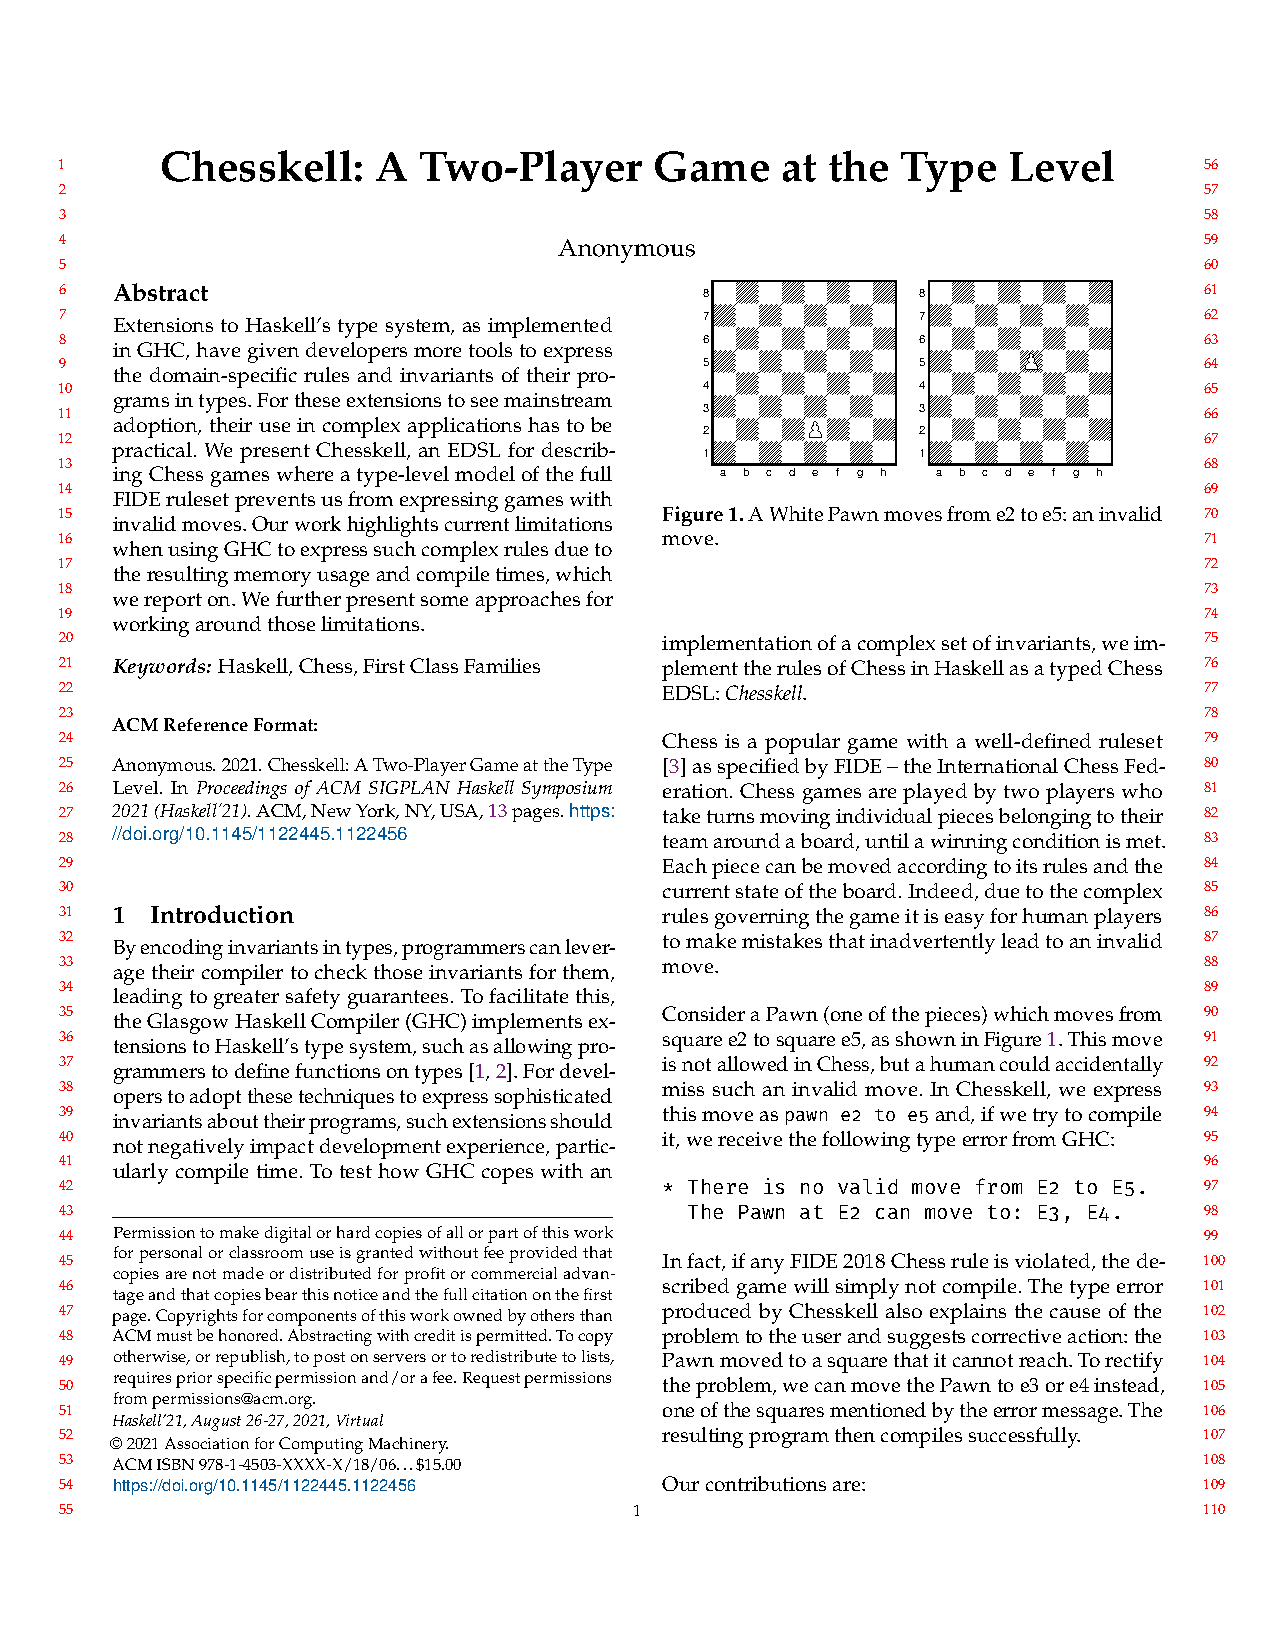
\includepdf[pages=-]{paper.pdf}

\end{document}